% =============================================================================
%  Používateľská príručka – Záhrada stratených ciest
%  Autor: Mykyta Olym, Počítačová grafika 2026/2027
% =============================================================================
\documentclass[11pt, a4paper]{article}
\newcommand{\druhprirucky}{Používateľská príručka}
% =============================================================================
%  Spoločné nastavenie všetkých troch dokumentov (preklad: latexmk -xelatex)
%  Záhrada stratených ciest – izometrické bludisko v knihe, Mykyta Olym, PG 2026/2027
% =============================================================================

% ---------------------------------------------------------------- údaje projektu
\newcommand{\nazovprojektu}{Záhrada stratených ciest}
\newcommand{\podnazovprojektu}{izometrické bludisko v knihe}
\newcommand{\predmet}{Počítačová grafika}
\newcommand{\skolskyrok}{2026/2027}
\newcommand{\ucitel}{Course Instructor}
\newcommand{\autor}{Mykyta Olym}
\newcommand{\verzia}{2.0}

% ---------------------------------------------------------------- jazyk a písmo
\usepackage{fontspec}
\usepackage{polyglossia}
\setdefaultlanguage{slovak}
\setmainfont{TeX Gyre Pagella}
\setsansfont{TeX Gyre Heros}
% neproporcionálne písmo zo šablóny KPI (priečinok fonts/)
\setmonofont{SourceCodePro}[
  Path = fonts/, Extension = .otf, Scale = 0.85,
  UprightFont = *-Regular, BoldFont = *-Bold,
  ItalicFont = *-Italic, BoldItalicFont = *-BoldItalic]

% ---------------------------------------------------------------- strana
\usepackage[a4paper, top=25mm, bottom=30mm, left=28mm, right=25mm]{geometry}
\usepackage{fancyhdr}
\pagestyle{fancy}
\fancyhf{}
\fancyhead[L]{\small\nazovprojektu}
\fancyhead[R]{\small\druhprirucky}
\fancyfoot[R]{\thepage}
\renewcommand{\headrulewidth}{0.4pt}
\setlength{\headheight}{14pt}
\setlength{\parindent}{0pt}
\setlength{\parskip}{0.55em}
\setlength{\emergencystretch}{3em}   % dlhé názvy radšej zalomiť než vytlačiť za okraj
% názvy súborov sa smú zalomiť za lomkou, bodkou alebo podčiarknutím
\usepackage[hyphens]{url}
\newcommand{\subor}[1]{\nolinkurl{#1}}

% ---------------------------------------------------------------- obsah, obrázky, tabuľky
\usepackage{graphicx}
\graphicspath{{obrazky/}}
\usepackage{booktabs, tabularx, array, longtable}
\usepackage{float}
\usepackage[font=small, labelfont=bf]{caption}
\usepackage{enumitem}
\setlist{itemsep=0.15em, topsep=0.3em}
\usepackage{xcolor}
\usepackage{csquotes}
\usepackage[style=iso-numeric, backend=biber, sorting=none]{biblatex}
\addbibresource{literatura.bib}
\usepackage[hidelinks]{hyperref}

% ---------------------------------------------------------------- titulná strana podľa pokynov
\newcommand{\titulnastrana}{%
  \begin{titlepage}
    \centering
    {\large Katedra počítačov a informatiky\\
      Fakulta elektrotechniky a informatiky\\
      Technická univerzita v Košiciach\par}
    \vspace*{\fill}
    {\Huge\bfseries \nazovprojektu\par}
    \vspace{0.4em}
    {\large \podnazovprojektu\par}
    \vspace{1.2em}
    {\Large \predmet\par}
    \vspace{3em}
    {\LARGE \druhprirucky\par}
    \vspace*{\fill}
    \begin{minipage}[t]{0.62\textwidth}
      \raggedright
      \begin{tabular}{@{}ll@{}}
        Šk. rok:       & \skolskyrok \\
        Meno učiteľa:  & \ucitel
      \end{tabular}
    \end{minipage}%
    \begin{minipage}[t]{0.38\textwidth}
      \raggedleft
      \begin{tabular}{@{}ll@{}}
        Autori: & \autor
      \end{tabular}
    \end{minipage}
  \end{titlepage}
  \setcounter{page}{1}%
}

% Obsah je podľa pokynov kapitola 1, preto skutočné kapitoly začínajú číslom 2.
\newcommand{\obsah}{%
  \renewcommand{\contentsname}{1\quad Obsah}%
  \tableofcontents
  \setcounter{section}{1}%
  \clearpage
}


\begin{document}
\titulnastrana
\obsah

% =============================================================================
\section{Funkcia programu}

Záhrada stratených ciest je hra o bludisku, rozprávaná ako kniha. Na stole leží kniha kresieb
babky Eleny; je zároveň menu aplikácie aj rozprávačom príbehu. Po otvorení knihy a začatí
príbehu sa kamera vnorí do kresby na strane a kresba ožije: je to izometricky nakreslená
usadlosť pri rieke so záhradným bludiskom zo živých plotov uprostred. Hráč prevedie postavu
bludiskom od vstupného oblúka k výstupnej bráne pri rieke, kde čaká babka; cestou môže
pozbierať tri zväzky kresieb, ktoré vietor rozfúkal po slepých uličkách. Na konci sa kamera
vráti do knihy a na poslednú stranu sa dopíše epilóg s~nakreslenou prejdenou cestou.

Program poskytuje tieto funkcie:
\begin{itemize}
  \item kniha ako menu: titulná strana s~údajmi o~projekte, obsah, strany Ako hrať, Nastavenia
    a O knihe; listy sa otáčajú ako papier, text sa píše ceruzkou,
  \item nové náhodné bludisko v~troch veľkostiach (5 × 5, 8 × 8 a 11 × 11 miestností),
  \item filmové scény: let kamery z~knihy do kresby a späť, titulok kapitoly, rozhovory
    s~postavami v~bublinách, čierne filmové pásy, titulky so spomienkami,
  \item hlasy: rozprávač číta prológ a epilóg, postavy hovoria (záhradník, babka, myšlienky
    postavy, spomienky) – text sa píše v~rytme reči, hudba pritom stíchne,
  \item pohyb postavy klávesnicou alebo kliknutím na miesto, kam má postava dôjsť,
  \item zbieranie troch zväzkov kresieb (každý odhalí jednu spomienku),
  \item nápovedu – ceruzka nakreslí cestu na najbližších krokoch k~cieľu,
  \item ukážku riešenia – postava sama dôjde k~bráne najkratšou cestou,
  \item záložku (pauzu) s~údajmi o~ceste, prípadne s~novým bludiskom,
  \item meranie času a krokov a ich porovnanie s~najkratšou cestou,
  \item živý svet: zámok s~fontánou, dedina s~domami, kostol, hospodársky dvor, pastvina, sad,
    rieka s~mostom, mólom a loďkou; ľudia, ktorí chodia po cestách a rozprávajú sa, zvieratá,
    motýle, vtáky, vlny na rieke, stromy vo vetre; dážď a slnko, hudba a zvuky.
\end{itemize}

\begin{figure}[H]
  \centering
  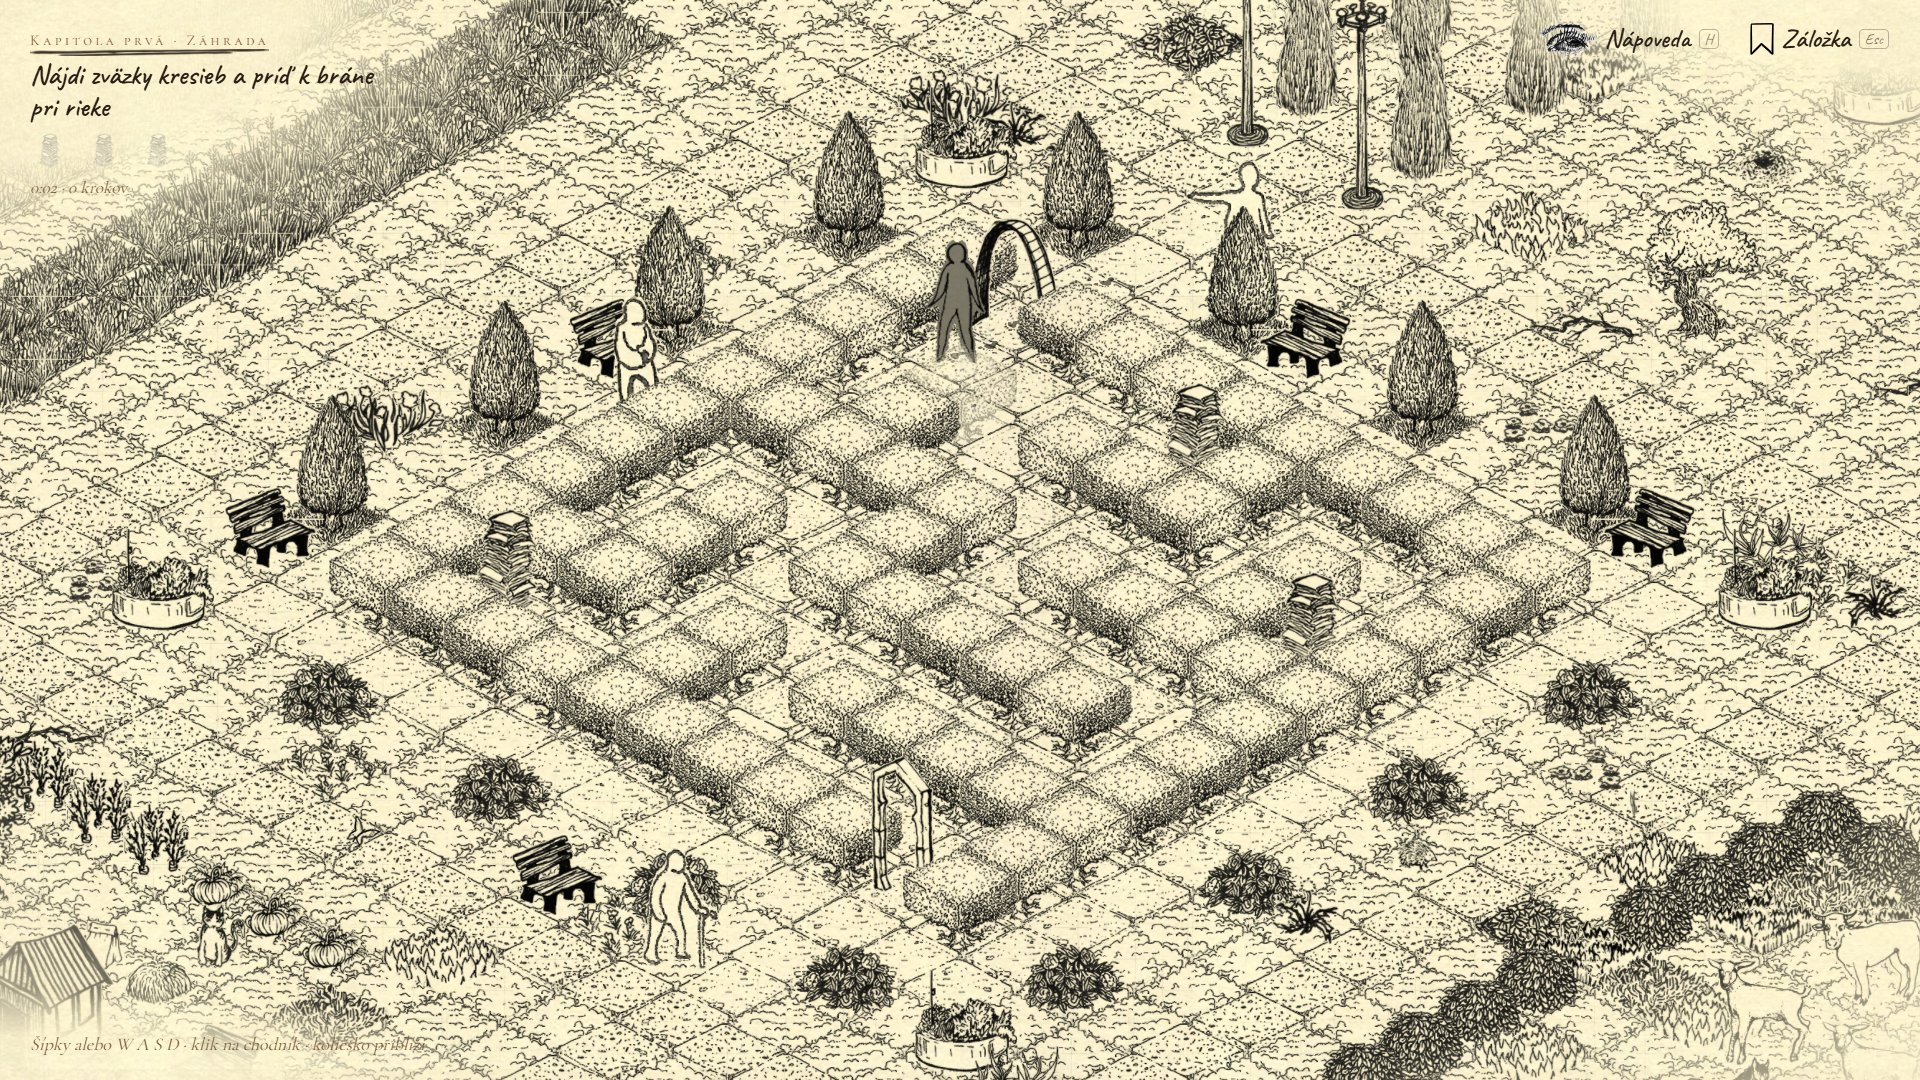
\includegraphics[width=\textwidth]{snimka-hra.jpg}
  \caption{Hra – postava v~bludisku}
\end{figure}

% =============================================================================
\section{Inštalácia programu}

\subsection{Súpis obsahu dodávky}

Program sa dodáva ako jeden balík \subor{Olym_PG1_20262027.zip} (bez hesla) na úložisku,
ktoré určí cvičiaci. Balík obsahuje jeden priečinok \subor{Olym_PG1_20262027}:

\begin{longtable}{@{}>{\raggedright\arraybackslash}p{0.44\textwidth}>{\raggedright\arraybackslash}p{0.51\textwidth}@{}}
  \toprule
  \textbf{Súbor alebo priečinok} & \textbf{Obsah} \\ \midrule
  \subor{index.html} & hlavná stránka aplikácie \\
  \subor{spustit.cmd} & spustenie cez lokálny webový server (Windows) \\
  \subor{licencie.txt} & autori a licencie kresieb, zvukov, písma a knižníc \\
  \subor{css/hra.css} & vzhľad knihy, stola a údajov počas hry \\
  \subor{js/*.js}, \subor{js/scenes/*.js} & program (zdrojové texty v~jazyku JavaScript) \\
  \subor{js/lib/phaser.min.js}, \subor{rot.min.js} & knižnice Phaser 4.2.1 a rot.js 2.2.1 \\
  \subor{texture/mesto.png}, \subor{mesto.json} & kresby sveta zbalené do jedného atlasu \\
  \subor{texture/kniha/} & kniha, doska, papier, stôl \\
  \subor{texture/ui/} & bublina, kvapka, ikony, ručne kreslené značky \\
  \subor{audio/} & hudba, zvuky prostredia a efekty (Ogg, MP3); v~\subor{audio/hlas/} hlasy rozprávača a postáv \\
  \subor{font/} & písma Caveat a Cormorant a ich licencie \\
  \subor{dokumentacia/Pouzivatelska_prirucka.pdf} & tento dokument \\
  \subor{dokumentacia/Systemova_prirucka.pdf} & dokument pre údržbu a ďalší vývoj programu \\
  \subor{dokumentacia/Zdrojove_texty.pdf} & výpis zdrojových textov \\ \bottomrule
\end{longtable}

\subsection{Požiadavky na technické prostriedky}

\begin{itemize}
  \item osobný počítač s~grafickou kartou s~podporou WebGL (integrovaná grafika, napr. Intel
    UHD Graphics 630, postačuje),
  \item operačná pamäť aspoň 4 GB, voľné miesto na disku približne 60 MB,
  \item monitor s~rozlíšením aspoň 1280 × 720 bodov (odporúča sa 1920 × 1080 alebo 2560 × 1440),
  \item klávesnica a myš, reproduktory alebo slúchadlá (nepovinné).
\end{itemize}

\subsection{Požiadavky na programové prostriedky}

\begin{itemize}
  \item operačný systém Windows 10 alebo 11 (pre súbor \subor{spustit.cmd}), prípadne Linux či macOS,
  \item webový prehliadač Google Chrome, Microsoft Edge alebo Mozilla Firefox vo verzii z~roku
    2024 alebo novšej so zapnutou hardvérovou akceleráciou,
  \item na spustenie lokálneho webového servera Python 3 alebo Node.js; inak vývojové prostredie
    WebStorm, ktoré má webový server zabudovaný,
  \item knižnice a písma sú súčasťou balíka, pripojenie na internet nie je potrebné.
\end{itemize}

\subsection{Vlastná inštalácia}

Program sa neinštaluje – stačí balík rozbaliť a spustiť. Postup:
\begin{enumerate}
  \item Balík \subor{Olym_PG1_20262027.zip} sa rozbalí do ľubovoľného priečinka.
    \emph{Správna odozva:} vznikne priečinok \subor{Olym_PG1_20262027} so súbormi podľa tabuľky vyššie.
    \emph{Chybová odozva:} operačný systém ohlási poškodený archív – balík treba stiahnuť znova.
  \item V~priečinku sa dvojklikom spustí súbor \subor{spustit.cmd}.
    \emph{Správna odozva:} otvorí sa okno príkazového riadka so spusteným webovým serverom
    a prehliadač otvorí adresu \subor{http://localhost:8137/}; po nápise „Načítava sa“ sa zo
    tmy vynorí stôl so zatvorenou knihou a kamera sa k~nej prisunie (obrázok~\ref{fig:stol}).
    \emph{Chybové odozvy:} hlásenie „Nenašiel sa Python ani Node.js“ – treba nainštalovať
    jeden z~nich alebo použiť postup v~bode 3; hlásenie Pythonu \texttt{OSError} s~kódom
    10048 – port 8137 používa iný program, ten treba zavrieť.
  \item Alternatíva bez súboru \subor{spustit.cmd}: priečinok sa otvorí vo WebStorme, na súbore
    \subor{index.html} sa zvolí \emph{Open In → Browser}.
  \item Aplikácia sa ukončí položkou „Zavrieť knihu“ v~obsahu knihy a zatvorením karty
    prehliadača. Webový server sa zastaví zatvorením okna príkazového riadka.
\end{enumerate}

Server spustený cez \subor{spustit.cmd} posiela prehliadaču hlavičku
\texttt{Cache-Control: no-store}, takže prehliadač vždy načíta aktuálne súbory. Ak sa súbor
\subor{index.html} otvorí priamo dvojklikom (adresa začína \subor{file://}), prehliadač
nenačíta moduly programu a namiesto knihy sa zobrazí návod (obrázok~\ref{fig:chyba-subor}).

\subsection{Spustenie DEMO verzie}

Samostatná demo verzia sa nedodáva. Priamo v~hre je funkcia \emph{Ukážka riešenia}
(v~záložke alebo kláves U), pri ktorej postava sama prejde bludiskom k~bráne a príbeh sa
dohrá až po epilóg. Táto funkcia je súčasťou dodaného programu a nevyžaduje samostatné video.

% =============================================================================
\section{Použitie programu}

\subsection{Popis jednotlivých funkcií a podfunkcií programu}

Po spustení sa zo tmy vynorí stôl so zatvorenou knihou (obrázok~\ref{fig:stol}). Kniha sa
otvorí kliknutím, klávesom Enter alebo medzerníkom: doska sa zdvihne a dopadne na stôl
a kniha sa otvorí na titulnej strane s~údajmi o~autorovi, katedre, fakulte, univerzite,
predmete a školskom roku. Na pravej strane je obsah (obrázok~\ref{fig:titul}). Položka obsahu,
na ktorú ukazuje myš, sa podčiarkne ceruzkou; kniha sa dá ovládať aj klávesnicou (Tab, Enter).

\begin{figure}[H]
  \centering
  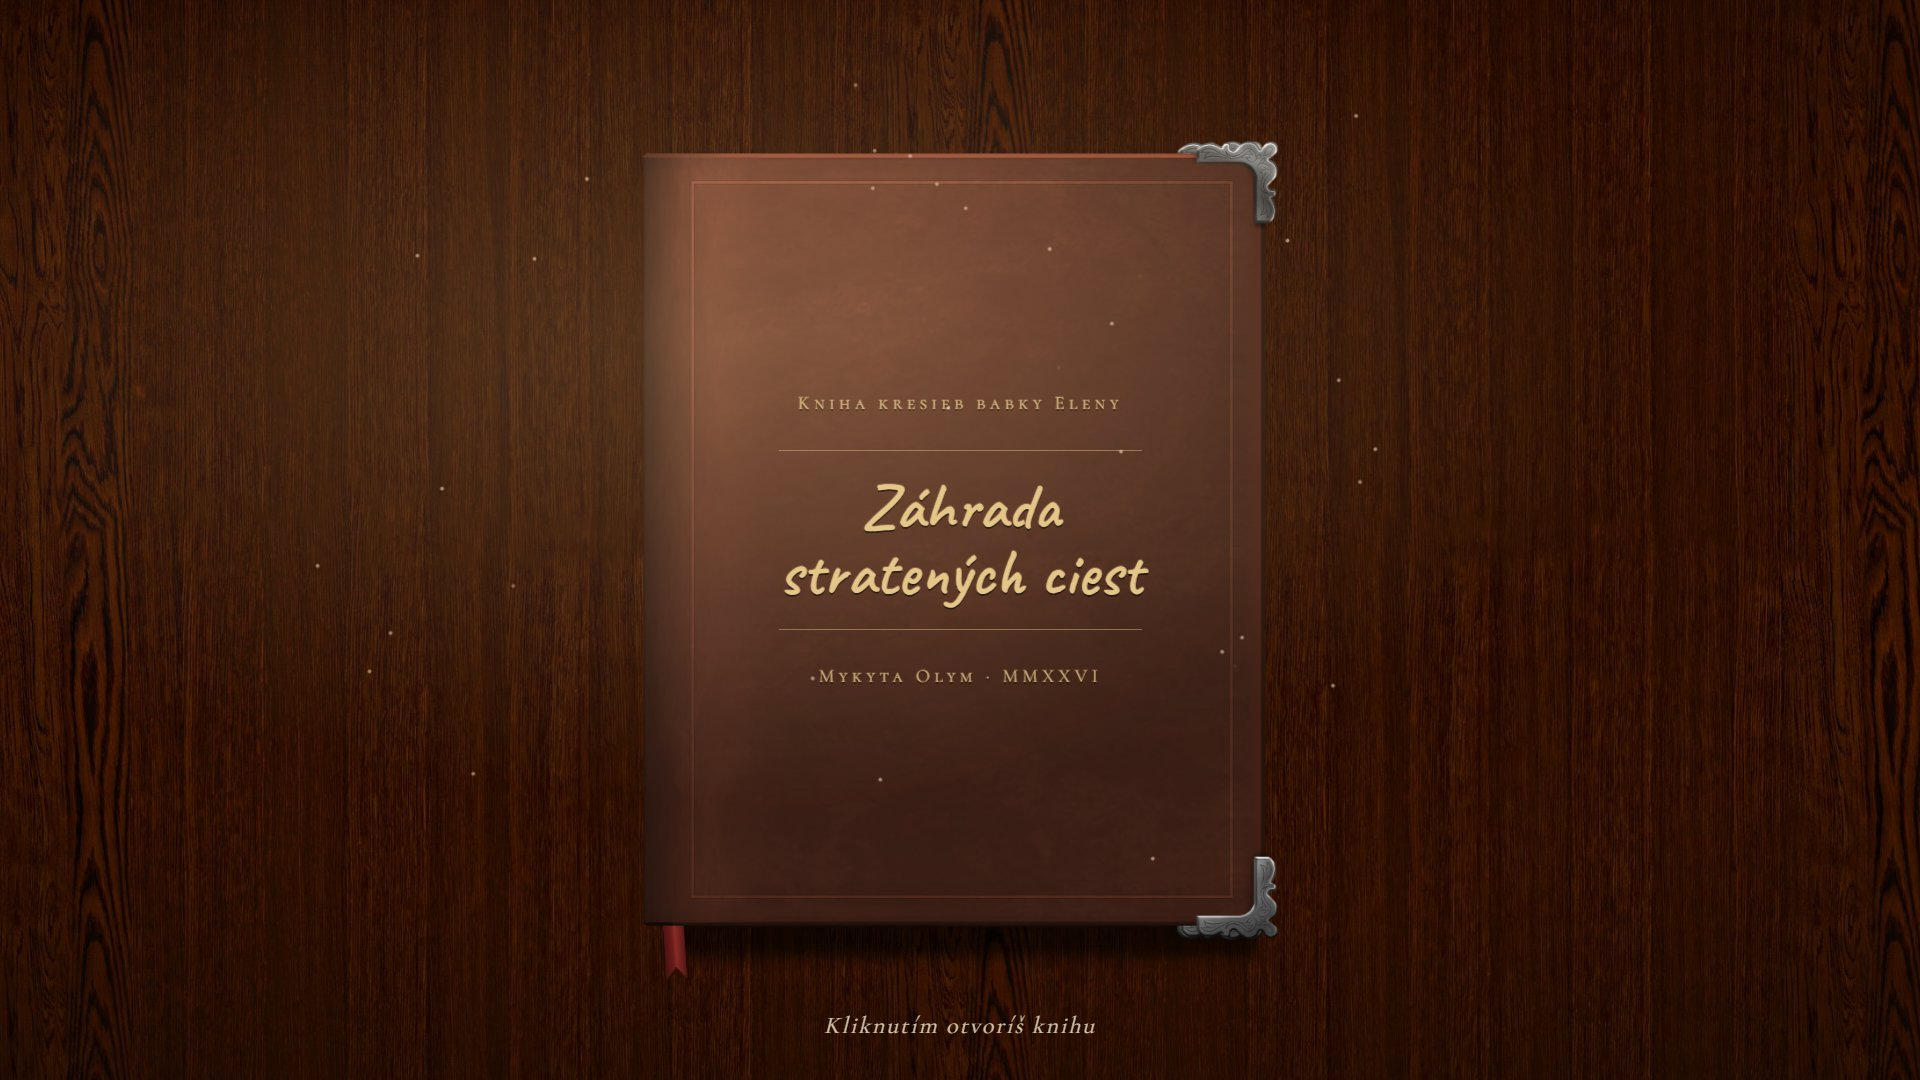
\includegraphics[width=0.85\textwidth]{snimka-stol.jpg}
  \caption{Stôl so zatvorenou knihou po spustení}\label{fig:stol}
\end{figure}

\begin{figure}[H]
  \centering
  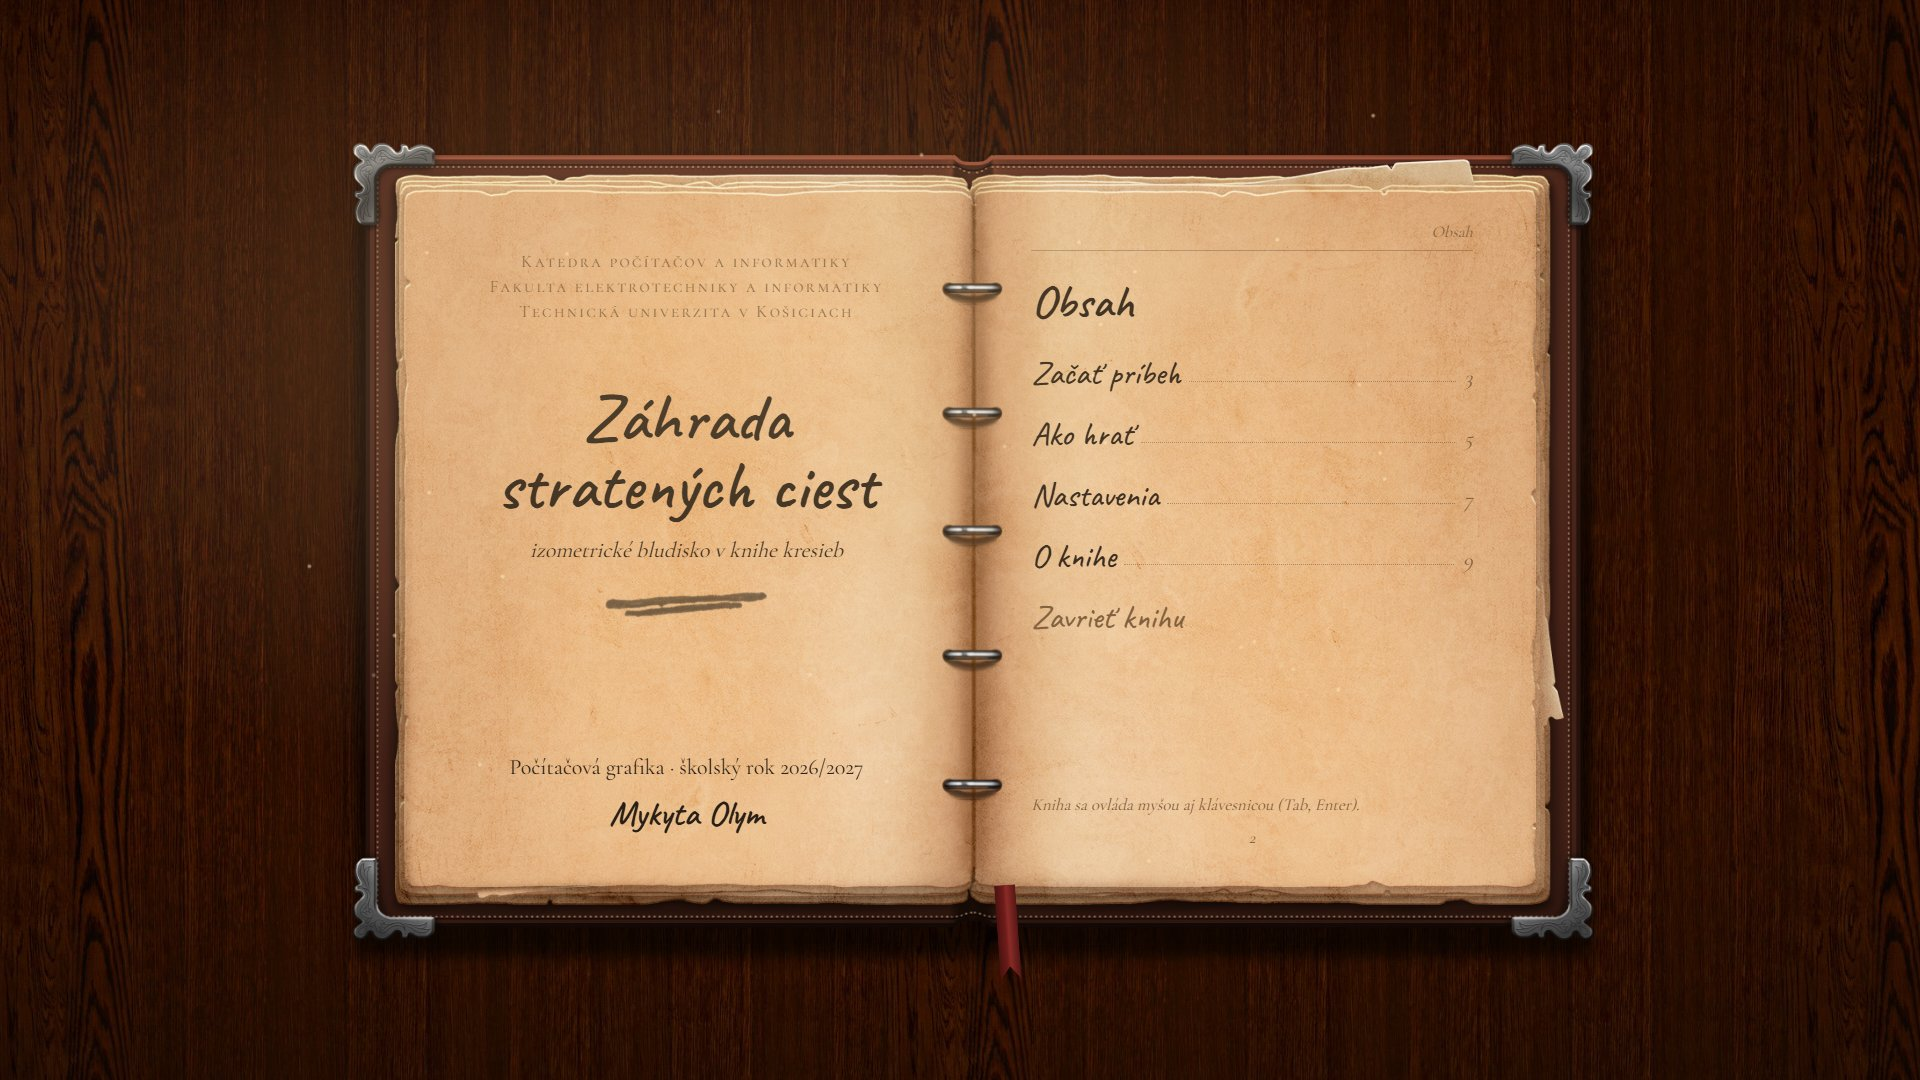
\includegraphics[width=0.85\textwidth]{snimka-titul.jpg}
  \caption{Titulná strana a obsah knihy}\label{fig:titul}
\end{figure}

\begin{table}[H]
  \centering
  \caption{Položky obsahu knihy}
  \begin{tabularx}{\textwidth}{@{}lX@{}}
    \toprule
    \textbf{Položka} & \textbf{Funkcia} \\ \midrule
    Začať príbeh & postaví nové bludisko zvolenej veľkosti a otočí list na prológ \\
    Ako hrať & strana s~prehľadom klávesov a myši a s~cieľom cesty \\
    Nastavenia & hudba, zvuky, hlasy a veľkosť bludiska (Malé, Stredné, Veľké) \\
    O knihe & údaje o~projekte a zoznam autorov kresieb, zvukov, písma a knižníc \\
    Zavrieť knihu & po potvrdení zavrie knihu a ukončí aplikáciu \\ \bottomrule
  \end{tabularx}
\end{table}

\subsection{Popis dialógu s používateľom}

Strom dialógu – prechody medzi stranami knihy a scénami a ovládacie prvky, ktoré ich vyvolajú –
je na obrázku~\ref{fig:obrazovky}. Každá nevratná akcia (zahodenie rozohranej cesty, návrat
na obsah počas hry, zavretie knihy) sa vykoná až po potvrdení: položka sa na strane prečiarkne
ceruzkou a pod ňou sa rukou dopíše „Naozaj? …“ s~voľbami „áno · nie“ (obrázok~\ref{fig:potvrdenie}).

\begin{figure}[H]
  \centering
  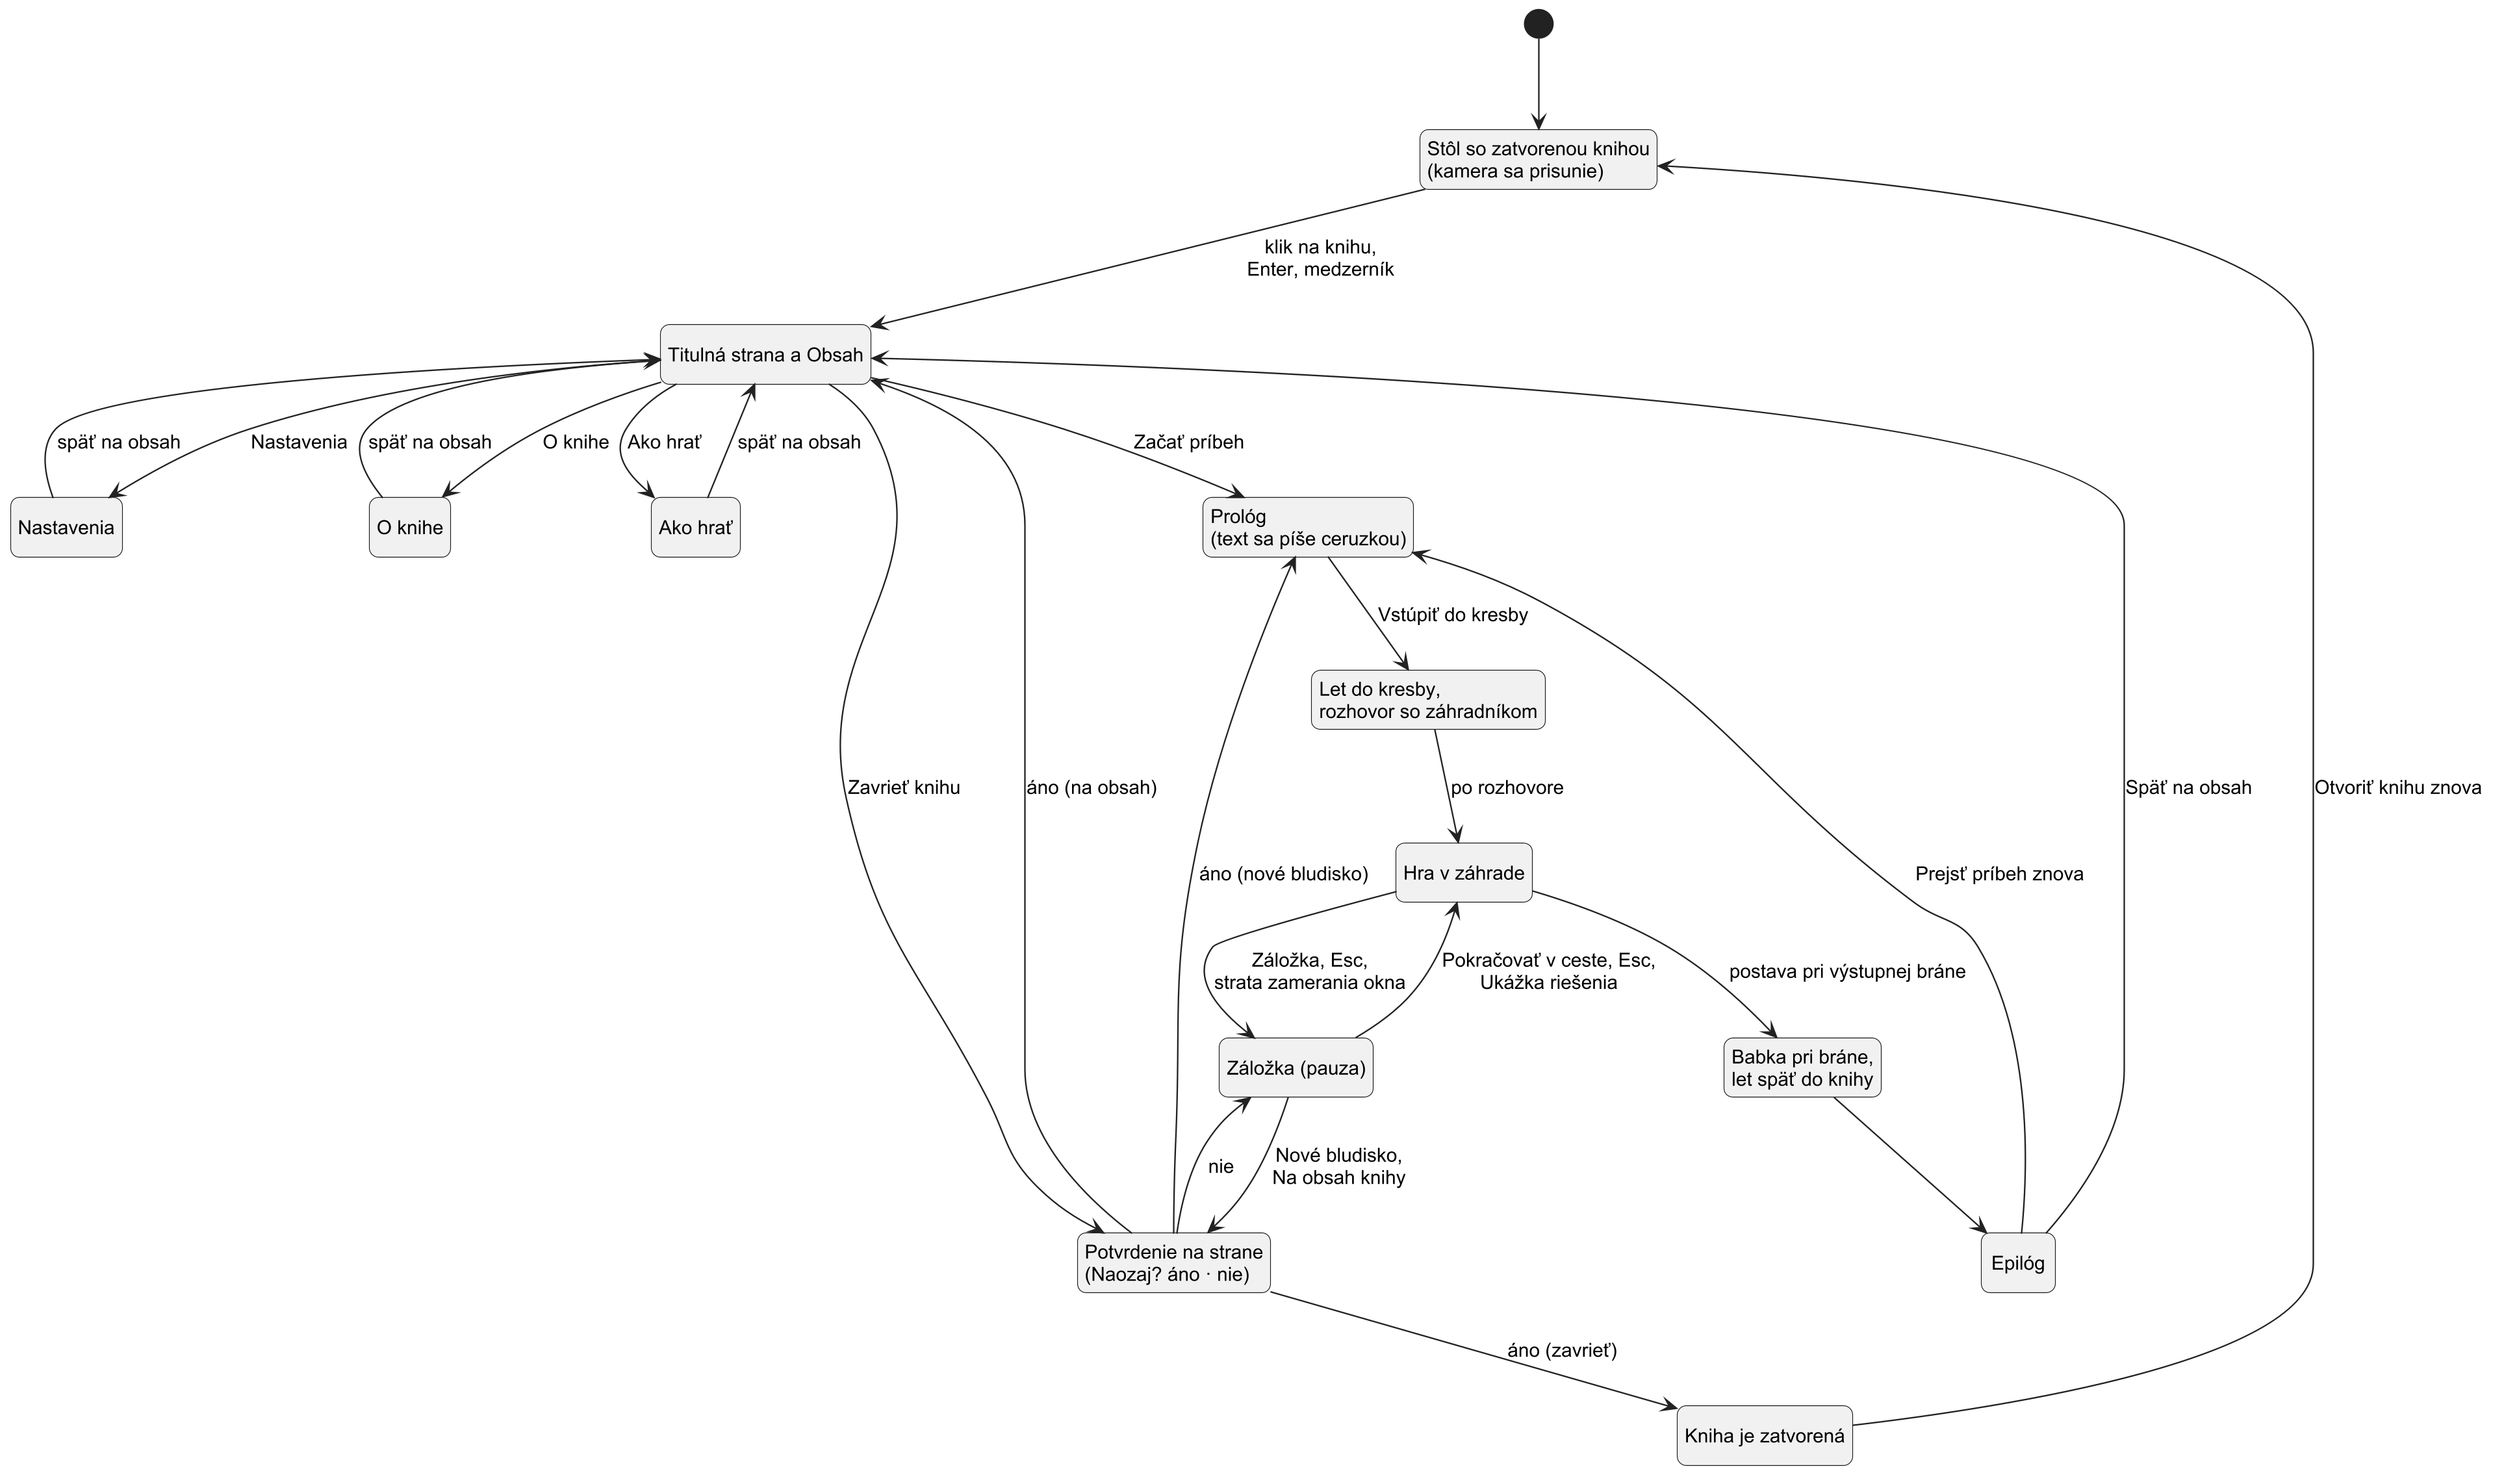
\includegraphics[width=\textwidth]{obrazovky.png}
  \caption{Strom dialógu: strany knihy, scény a prechody medzi nimi}\label{fig:obrazovky}
\end{figure}

\begin{figure}[H]
  \centering
  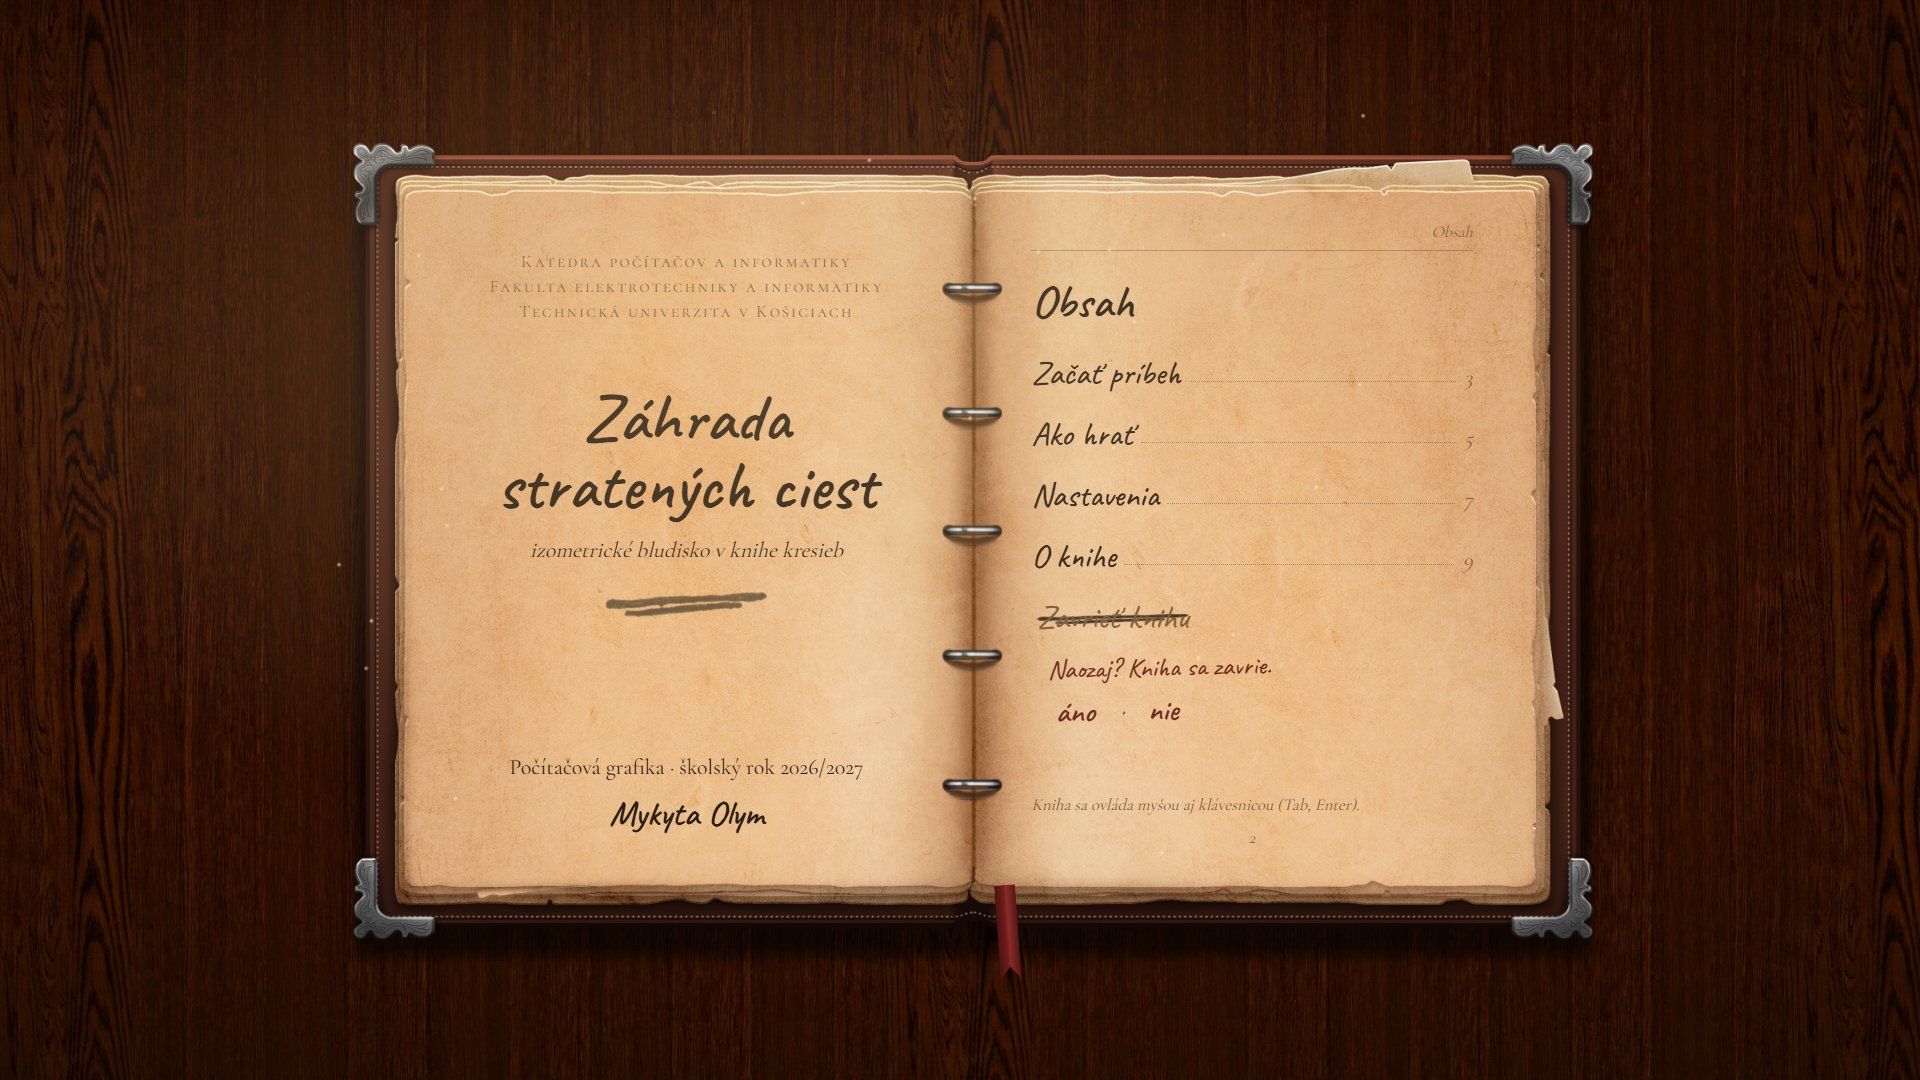
\includegraphics[width=0.85\textwidth]{snimka-potvrdenie.jpg}
  \caption{Potvrdenie nevratnej akcie priamo na strane knihy}\label{fig:potvrdenie}
\end{figure}

\subsection{Popis podfunkcií}

\paragraph{Prológ a vstup do kresby.} Po zvolení „Začať príbeh“ sa list otočí na prológ.
Kresba dediny sa vpije do papiera, rozprávač prológ číta a text sa píše slovo po slove presne
v~rytme jeho reči (kliknutie na knihu dopíše text naraz a rozprávač stíchne). Tlačidlom „Vstúpiť do kresby“ sa kamera začne približovať ku kresbe;
kresba sa uprostred letu zmení na živý svet a kamera pokračuje až k~vstupnej bráne, kde čaká
záhradník Matej. Počas letu rozprávač ohlási kapitolu. Postavy hovoria nahlas, text bubliny
sa píše v~rytme reči a keď veta dozneje, bublina sa po chvíli sama zavrie. Kliknutím,
medzerníkom alebo klávesom Enter sa rozhovor dá zrýchliť (prvé stlačenie vetu dopíše a hlas
stíši, druhé bublinu zavrie). Po rozhovore postava vojde oblúkom do bludiska,
kamera sa pritom vznesie nad celé bludisko a začne sa hra.

\paragraph{Hra.} V~ľavom hornom rohu je lístok s~úlohou, tromi miestami pre zväzky kresieb,
časom a počtom krokov; v~pravom hornom rohu tlačidlá Nápoveda a Záložka; dole stručná rada
k~ovládaniu, ktorá po prvom kroku zmizne. Kurzor nad voľnou bunkou bludiska ju zakrúžkuje
ceruzkou. Po kliknutí ostane na cieli výraznejší krúžok, ktorý jemne dýcha, kým tam postava
nedôjde; keď sú všetky zväzky pokope, ceruzka zakrúžkuje aj výstupnú bránu. Krúžky sú
nakreslené akoby na papier knihy, preto ich nezakryje ani vysoký živý plot.

\begin{table}[H]
  \centering
  \caption{Ovládanie počas hry}
  \begin{tabularx}{\textwidth}{@{}lX@{}}
    \toprule
    \textbf{Ovládací prvok} & \textbf{Funkcia} \\ \midrule
    ↑ alebo W & krok vpravo hore \\
    → alebo D & krok vpravo dole \\
    ↓ alebo S & krok vľavo dole \\
    ← alebo A & krok vľavo hore \\
    držaný kláves & postava kráča ďalej, kým je kláves stlačený \\
    klik na chodník & postava dôjde na zvolené miesto najkratšou cestou \\
    koliesko myši & priblíženie (kamera potom sleduje postavu) a oddialenie na celé bludisko \\
    Nápoveda (H) & ceruzka nakreslí cestu na 12 krokoch k~najbližšiemu cieľu \\
    Záložka (Esc) & zastaví čas a vysunie knihu so záložkou \\
    U & ukážka riešenia – postava sama dôjde k~bráne \\
    medzerník, Enter, klik & dopíše vetu rozhovoru, ďalšie stlačenie ju zavrie (inak sa zavrie sama) \\
    F & prepne celú obrazovku \\ \bottomrule
  \end{tabularx}
\end{table}

\paragraph{Myšlienky postavy.} Postava si všíma okolie. Keď príde k~studni, kamennému stĺpu
alebo záhonu v~zákutí bludiska, otočí sa k~nemu a nad hlavou sa jej objaví bublina s~myšlienkou
o~ňom, ktorú povie nahlas; vlastné myšlienky má aj v~slepej uličke, po opakovanom náraze do živého plota a pred
výstupnou bránou, ak ešte nemá všetky zväzky. Na studňu, stĺp ani záhon sa vstúpiť nedá.
Myšlienka hru nezastaví – po chvíli sama vybledne.

\paragraph{Zväzky kresieb.} Na troch miestach bludiska ležia zväzky kresieb. Keď na ne postava
vstúpi, zväzok vyletí na lístok a dole sa zobrazí spomienka babky Eleny, ktorú prečíta jej hlas. Po druhom zväzku sa
spustí dážď (na cestách sa objavia mláky, motýle sa schovajú), po chvíli sa vyjasní. Zväzky nie
sú povinné – bez nich sa však príbeh skončí inými vetami.

\paragraph{Záložka.} Hra sa pozastaví tlačidlom, klávesom Esc alebo sama, keď okno prehliadača
stratí zameranie. Svet zošedne ako zastavený filmový záber a zdola sa vysunie kniha otvorená na
strane so záložkou (obrázok~\ref{fig:zalozka}). Ľavá strana ukazuje čas, počet krokov a nájdené
zväzky, pravá ponúka „Pokračovať v~ceste“, „Ukážka riešenia“, „Nové bludisko“ a „Na obsah knihy“
(posledné dve po potvrdení).

\paragraph{Koniec cesty.} Keď postava vyjde výstupnou bránou, prejde k~babke, od radosti poskočí
a babka prehovorí. Kamera ukáže celé bludisko a pero červeným atramentom nakreslí prejdenú cestu;
na jej konci zaznie melódia, z~brány vyletia motýle a vtáky a prefúkne vietor. Potom sa kamera
vzdiali nad celý ostrov a ďalej až ku knihe na stole – svet sa vráti do kresby. Rozprávač
číta epilóg, kým sa text dopisuje; na kresbe je atramentom prejdená cesta.
Epilóg uvádza čas v~záhrade, počet krokov, dĺžku najkratšej cesty a počet nájdených zväzkov
a ponúka „Prejsť príbeh znova“ a „Späť na obsah“.

\paragraph{Nastavenia.} Prepínače „Hudba“, „Zvuky záhrady a knihy“ a „Hlasy rozprávača
a postáv“ platia ihneď (bez hlasov sa text píše rovnomerne a čas na čítanie sa riadi dĺžkou vety), veľkosť
bludiska pre najbližší príbeh. Kniha si nastavenia zapamätá.

\paragraph{Zavretie knihy.} Po potvrdení sa ľavá strana zdvihne spolu s~doskou, kniha sa zavrie,
svetlo zhasne a zobrazí sa „Kniha je zatvorená“ s~tlačidlom „Otvoriť knihu znova“.

% =============================================================================
\section{Popis vstupných a výstupných súborov}

Program nepracuje so súbormi používateľa. Jediné uložené údaje sú nastavenia, ktoré sa ukladajú
do úložiska prehliadača (\texttt{localStorage}) pod kľúčom \subor{zahrada-stratenych-ciest}
vo formáte JSON, napríklad \subor{{"music": true, "sounds": true, "size": "stredne"}}.
V~súkromnom režime prehliadača sa nastavenia neuložia a pri ďalšom spustení platia predvolené
hodnoty (hudba, zvuky a hlasy zapnuté, stredné bludisko).

Pracovné súbory programu (atlas kresieb \subor{texture/mesto.json} vo formáte JSON Hash,
obrázky PNG, JPEG a SVG, zvuky Ogg a MP3, písma TTF) používateľ nemení.

% =============================================================================
\section{Obmedzenia programu}

\begin{itemize}
  \item hru hrá jeden hráč; rozohraná cesta sa neukladá, každé nové bludisko je náhodné,
  \item veľkosti bludiska sú tri: 11 × 11, 17 × 17 a 23 × 23 buniek mriežky,
  \item program vyžaduje WebGL; bez grafickej akcelerácie môžu byť animácie trhané,
  \item hudba, zvuky a hlasy sa spustia až po prvom kliknutí alebo stlačení klávesu (prehliadače bez
    toho zvuk nepovolia),
  \item aplikácia je určená pre klávesnicu a myš, dotykové ovládanie nie je prispôsobené,
  \item texty sú v~slovenčine.
\end{itemize}

% =============================================================================
\section{Chybové hlásenia}

\begin{table}[H]
  \centering
  \caption{Chybové hlásenia aplikácie}
  \begin{tabularx}{\textwidth}{@{}>{\raggedright}p{0.38\textwidth}X@{}}
    \toprule
    \textbf{Hlásenie} & \textbf{Príčina a riešenie} \\ \midrule
    Hru treba otvoriť cez webový server: spustite súbor spustit.cmd alebo index.html vo WebStorme. &
      súbor \subor{index.html} bol otvorený priamo z~disku; hru treba spustiť podľa kapitoly 3.4 \\
    Prehliadač nepodporuje WebGL. Použite aktuálny Chrome, Edge alebo Firefox so zapnutou hardvérovou akceleráciou. &
      prehliadač je starý alebo má vypnutú hardvérovú akceleráciu \\
    Nepodarilo sa načítať: \emph{zoznam súborov}. Rozbaľte celý balík znova a spustite hru cez spustit.cmd. &
      v~priečinku chýba alebo je poškodený súbor s~kresbami či zvukmi \\
    Aplikácia potrebuje zapnutý JavaScript. & v~prehliadači je vypnutý JavaScript \\ \bottomrule
  \end{tabularx}
\end{table}

\begin{table}[H]
  \centering
  \caption{Hlásenia operačného systému a prehliadača}
  \begin{tabularx}{\textwidth}{@{}>{\raggedright}p{0.38\textwidth}X@{}}
    \toprule
    \textbf{Hlásenie} & \textbf{Príčina a riešenie} \\ \midrule
    Nenašiel sa Python ani Node.js. & \subor{spustit.cmd} nenašiel program pre webový server;
      nainštalovať Python 3 alebo Node.js, alebo použiť WebStorm \\
    OSError: [WinError 10048] & port 8137 už používa iný program; zavrieť ho a spustiť znova \\
    Opustiť stránku? (otázka prehliadača) & karta sa zatvára počas rozohranej cesty; prehliadač
      sa pýta, či ju naozaj zahodiť \\ \bottomrule
  \end{tabularx}
\end{table}

\begin{figure}[H]
  \centering
  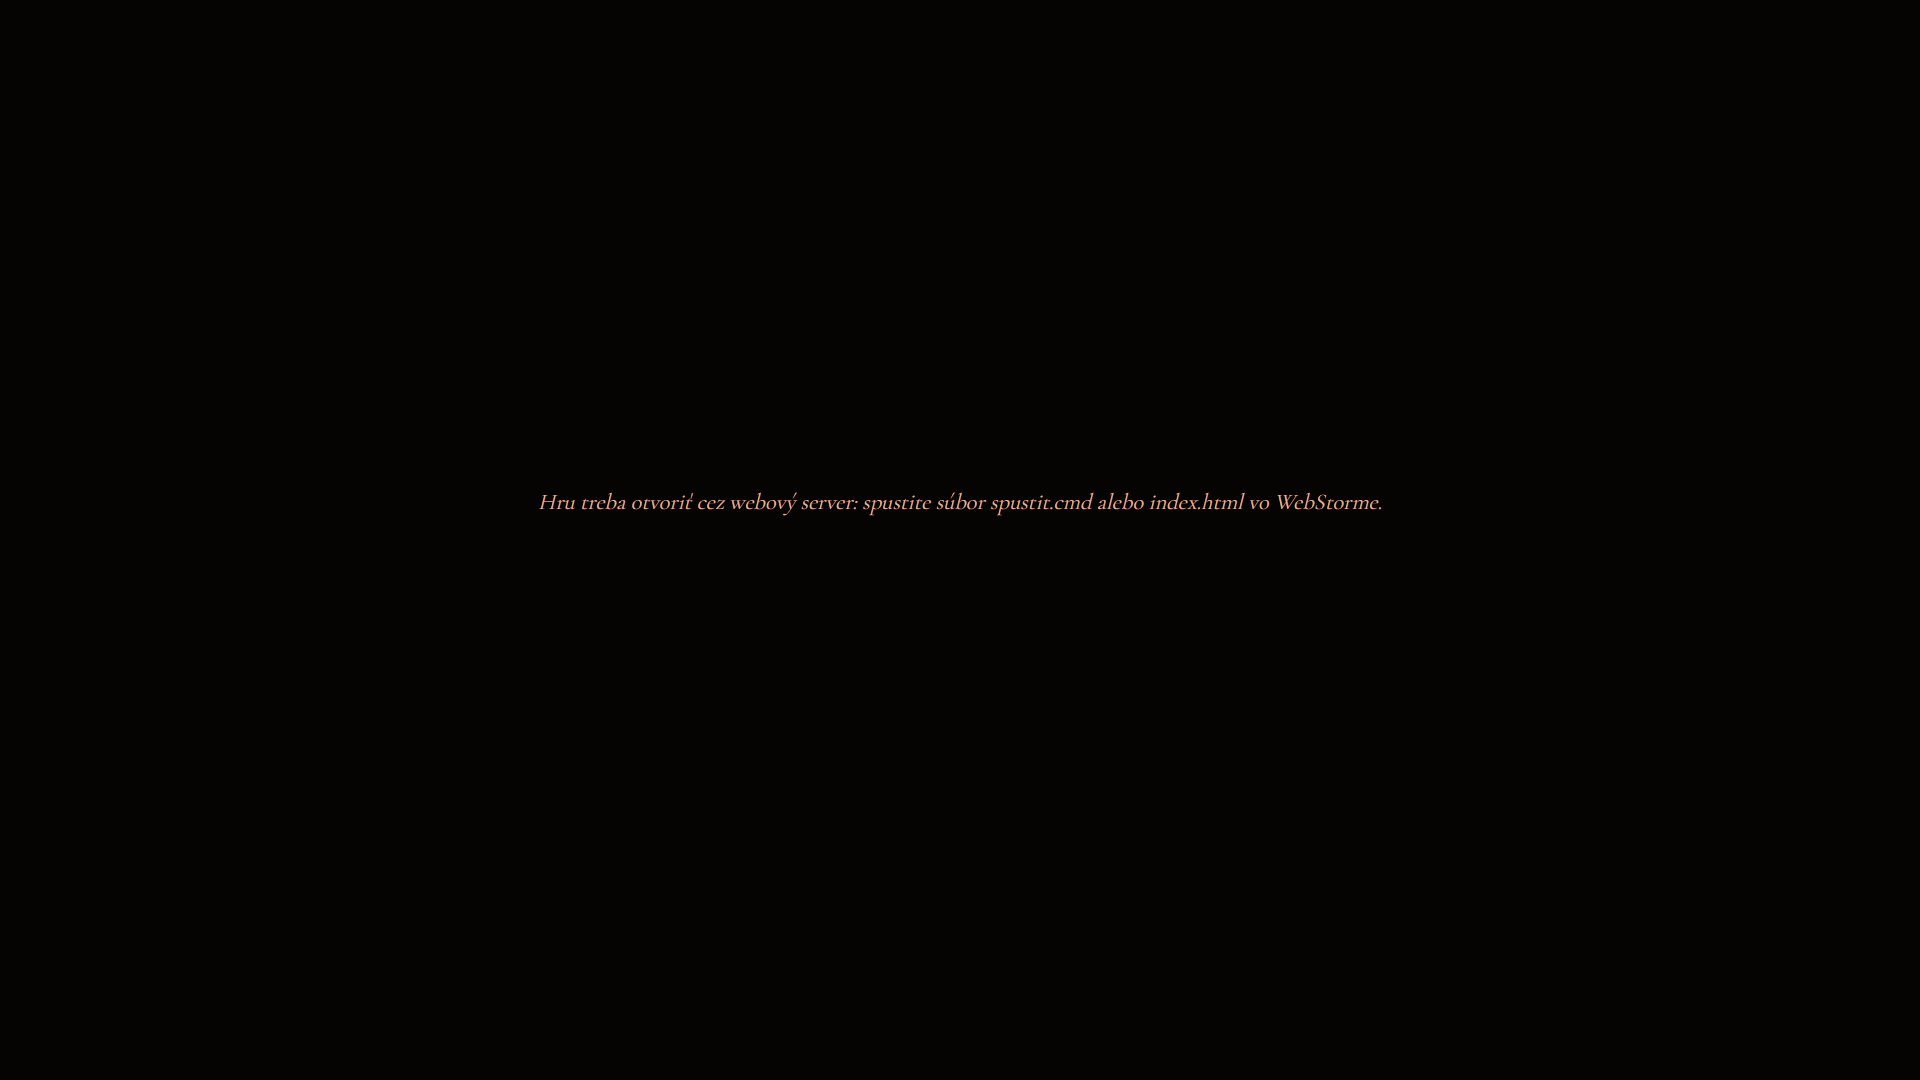
\includegraphics[width=0.85\textwidth]{snimka-chyba-subor.jpg}
  \caption{Hlásenie pri otvorení súboru priamo z~disku}\label{fig:chyba-subor}
\end{figure}

% =============================================================================
\section{Príklad použitia}

Nasledujúce snímky zachytávajú jeden príbeh od otvorenia knihy po jej zavretie.

\begin{figure}[H]
  \centering
  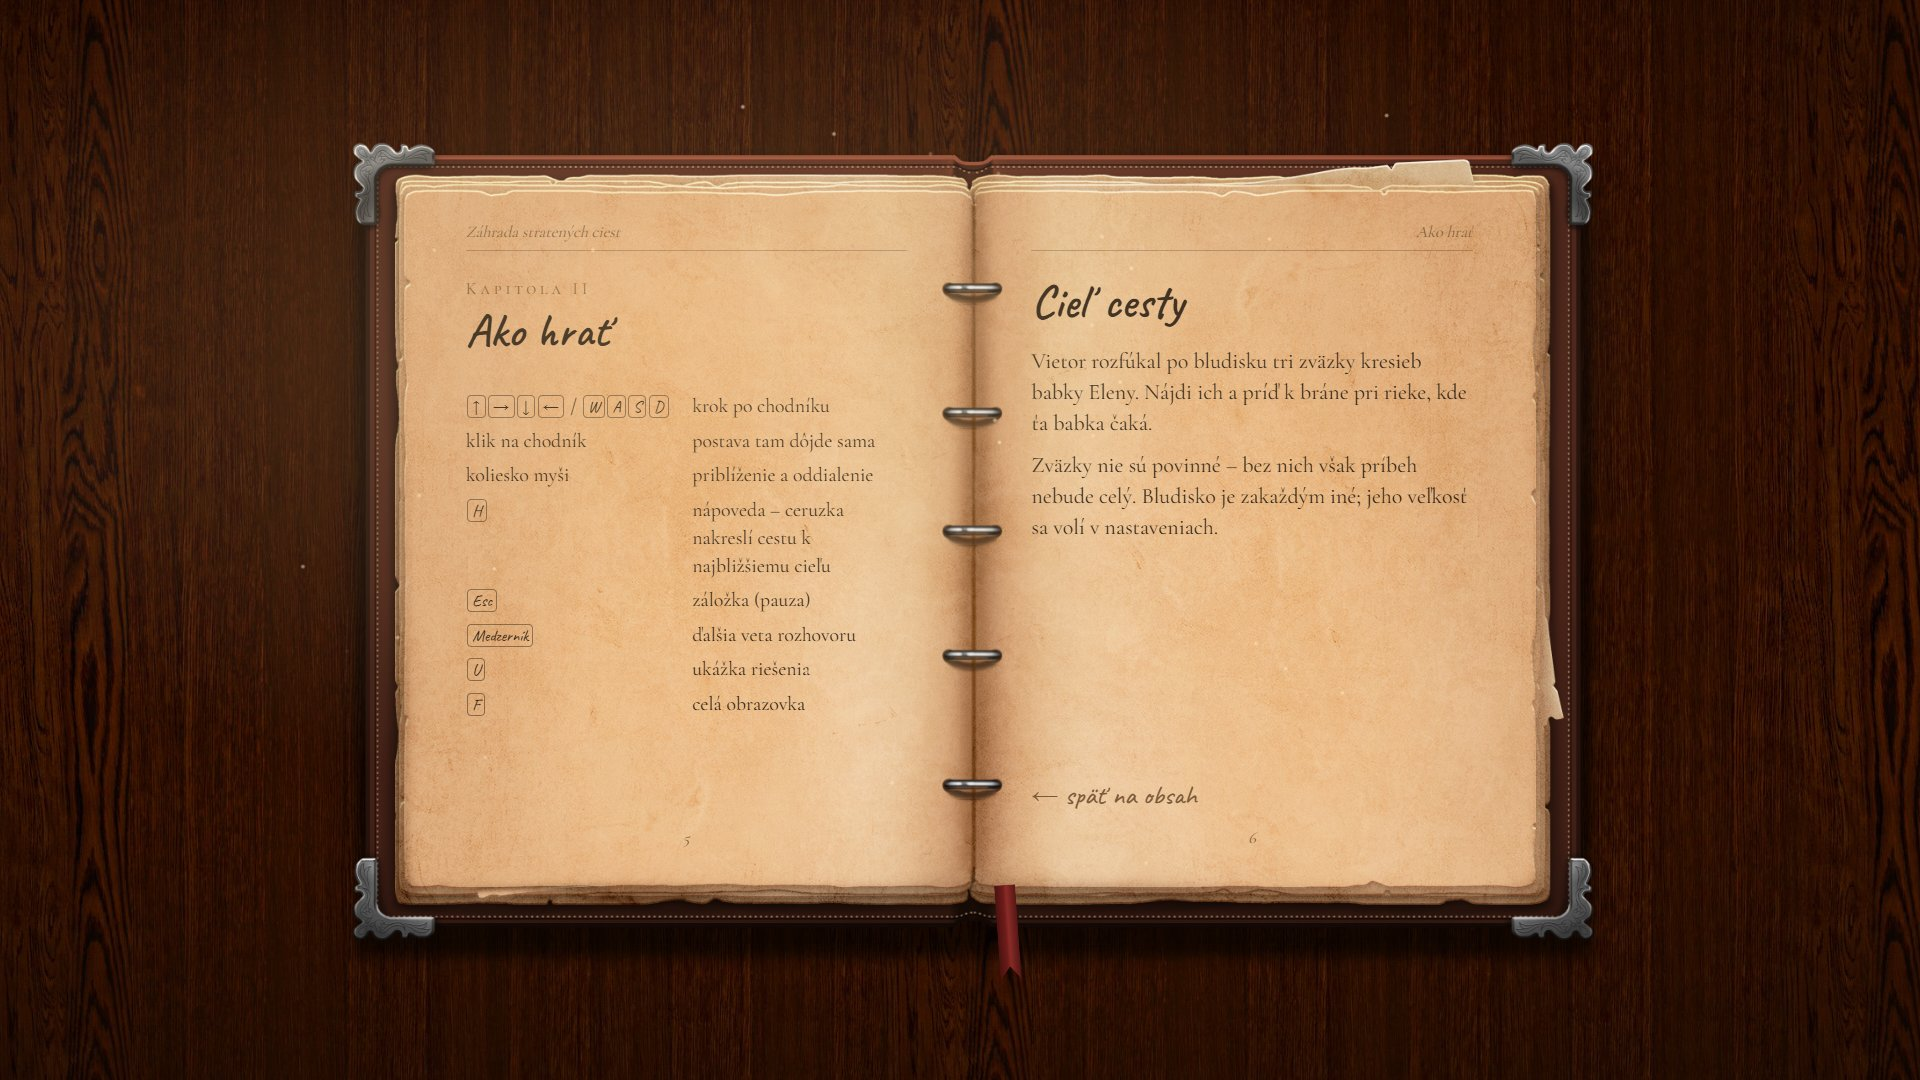
\includegraphics[width=0.85\textwidth]{snimka-navod.jpg}
  \caption{Strana Ako hrať}
\end{figure}

\begin{figure}[H]
  \centering
  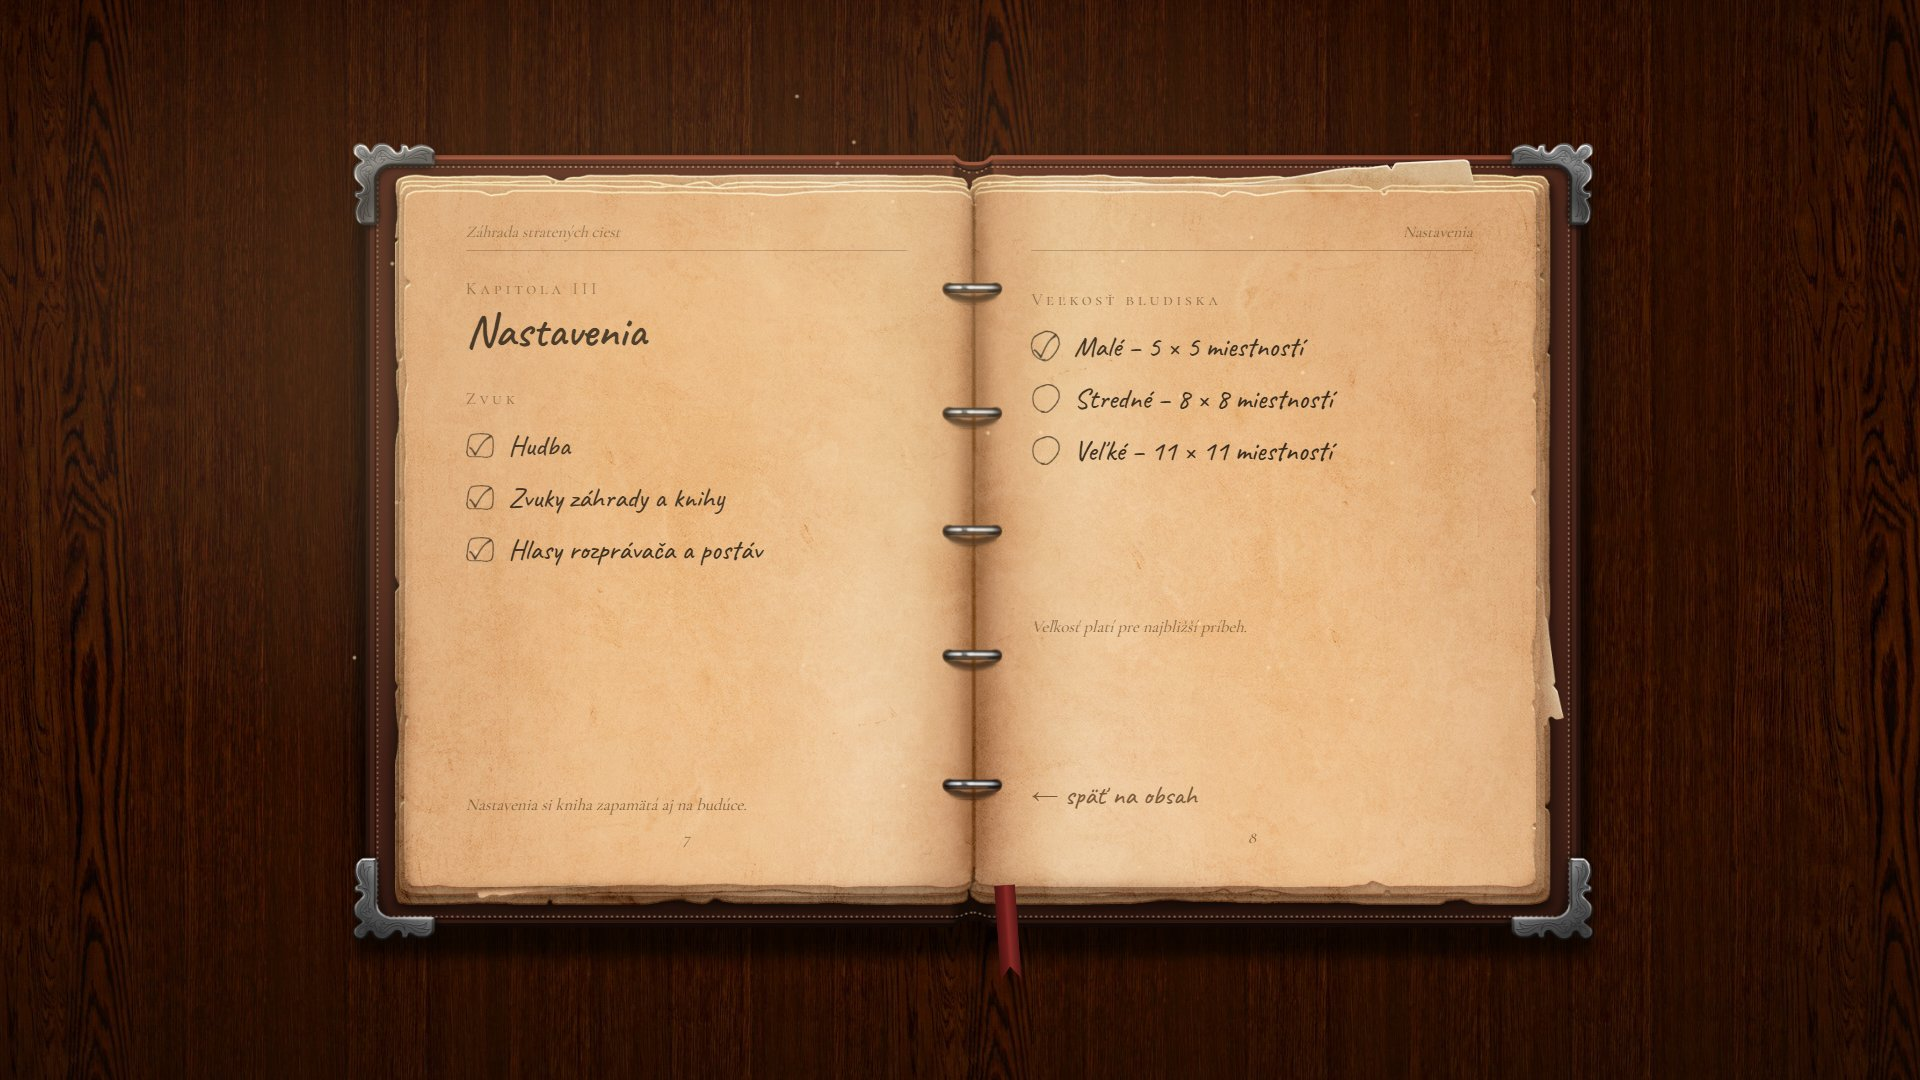
\includegraphics[width=0.85\textwidth]{snimka-nastavenia.jpg}
  \caption{Nastavenia – zvolené malé bludisko}
\end{figure}

\begin{figure}[H]
  \centering
  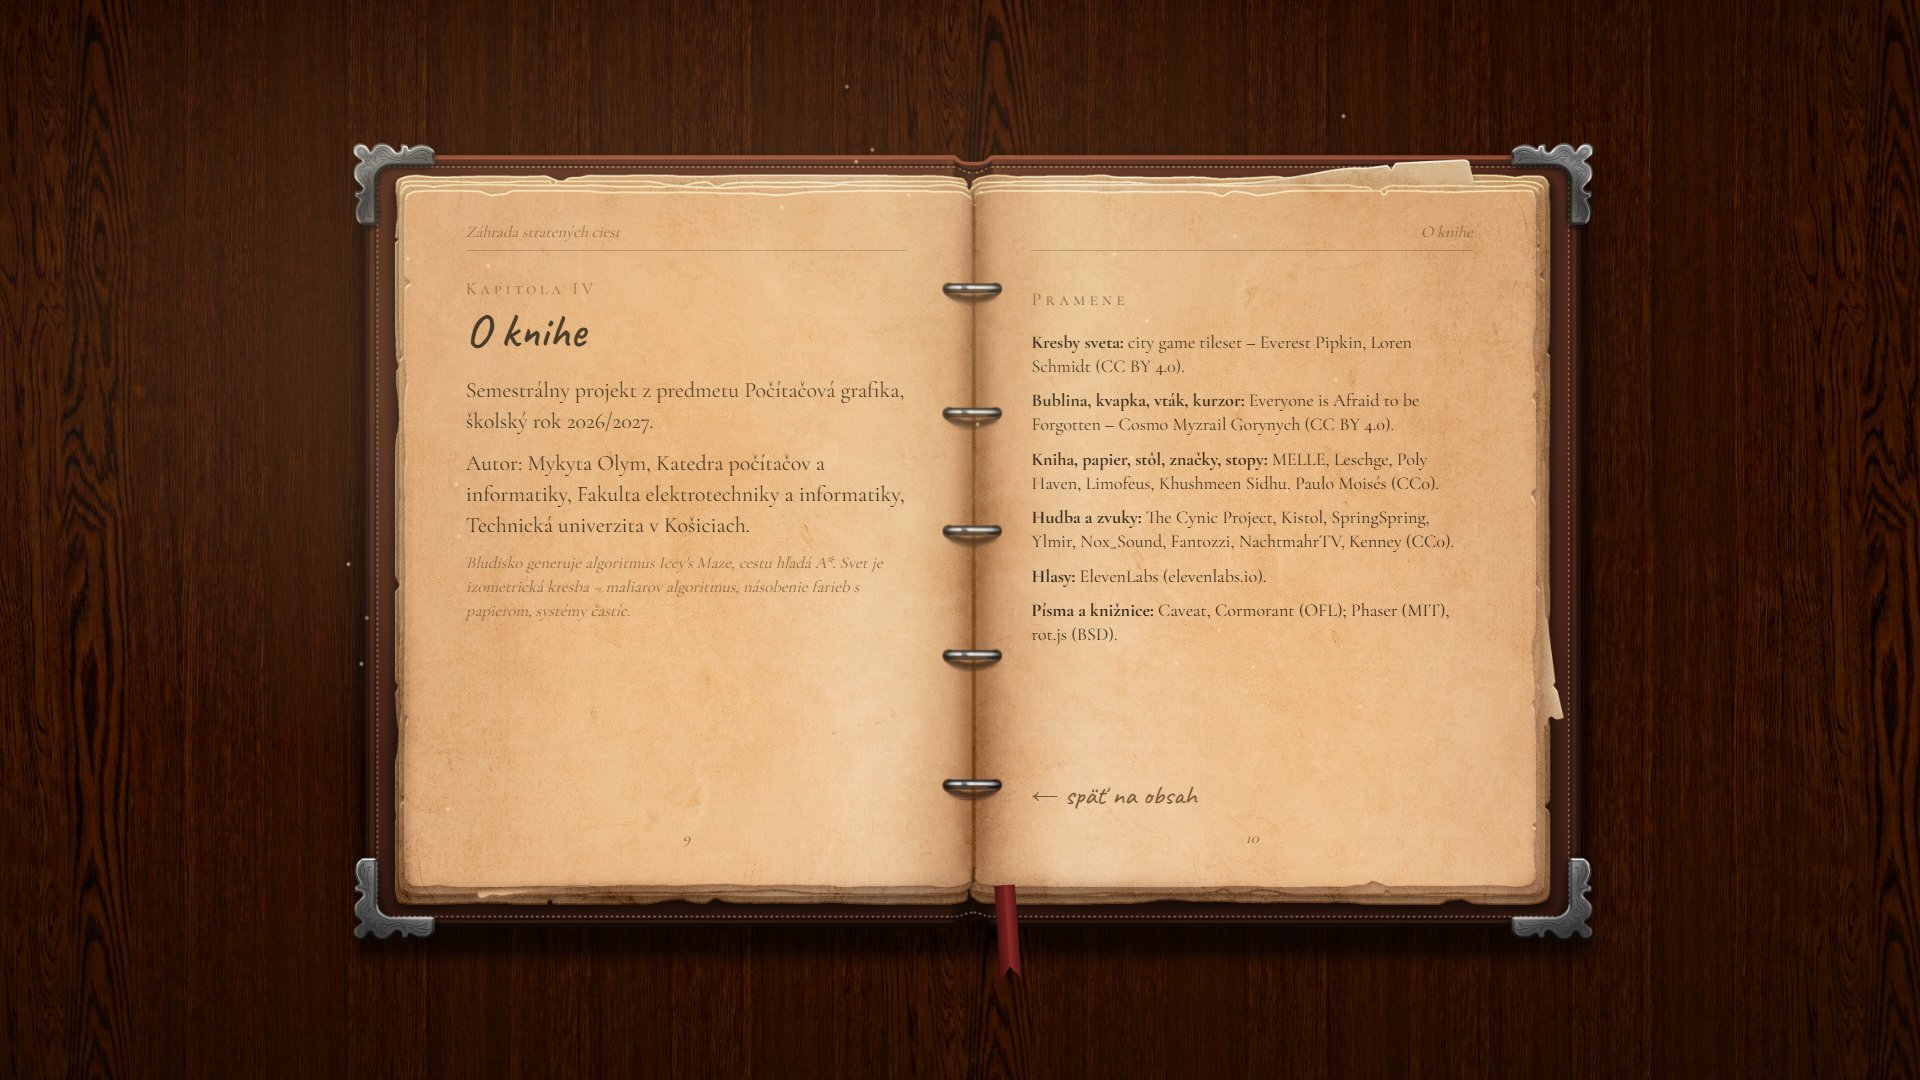
\includegraphics[width=0.85\textwidth]{snimka-o-knihe.jpg}
  \caption{Strana O knihe}
\end{figure}

\begin{figure}[H]
  \centering
  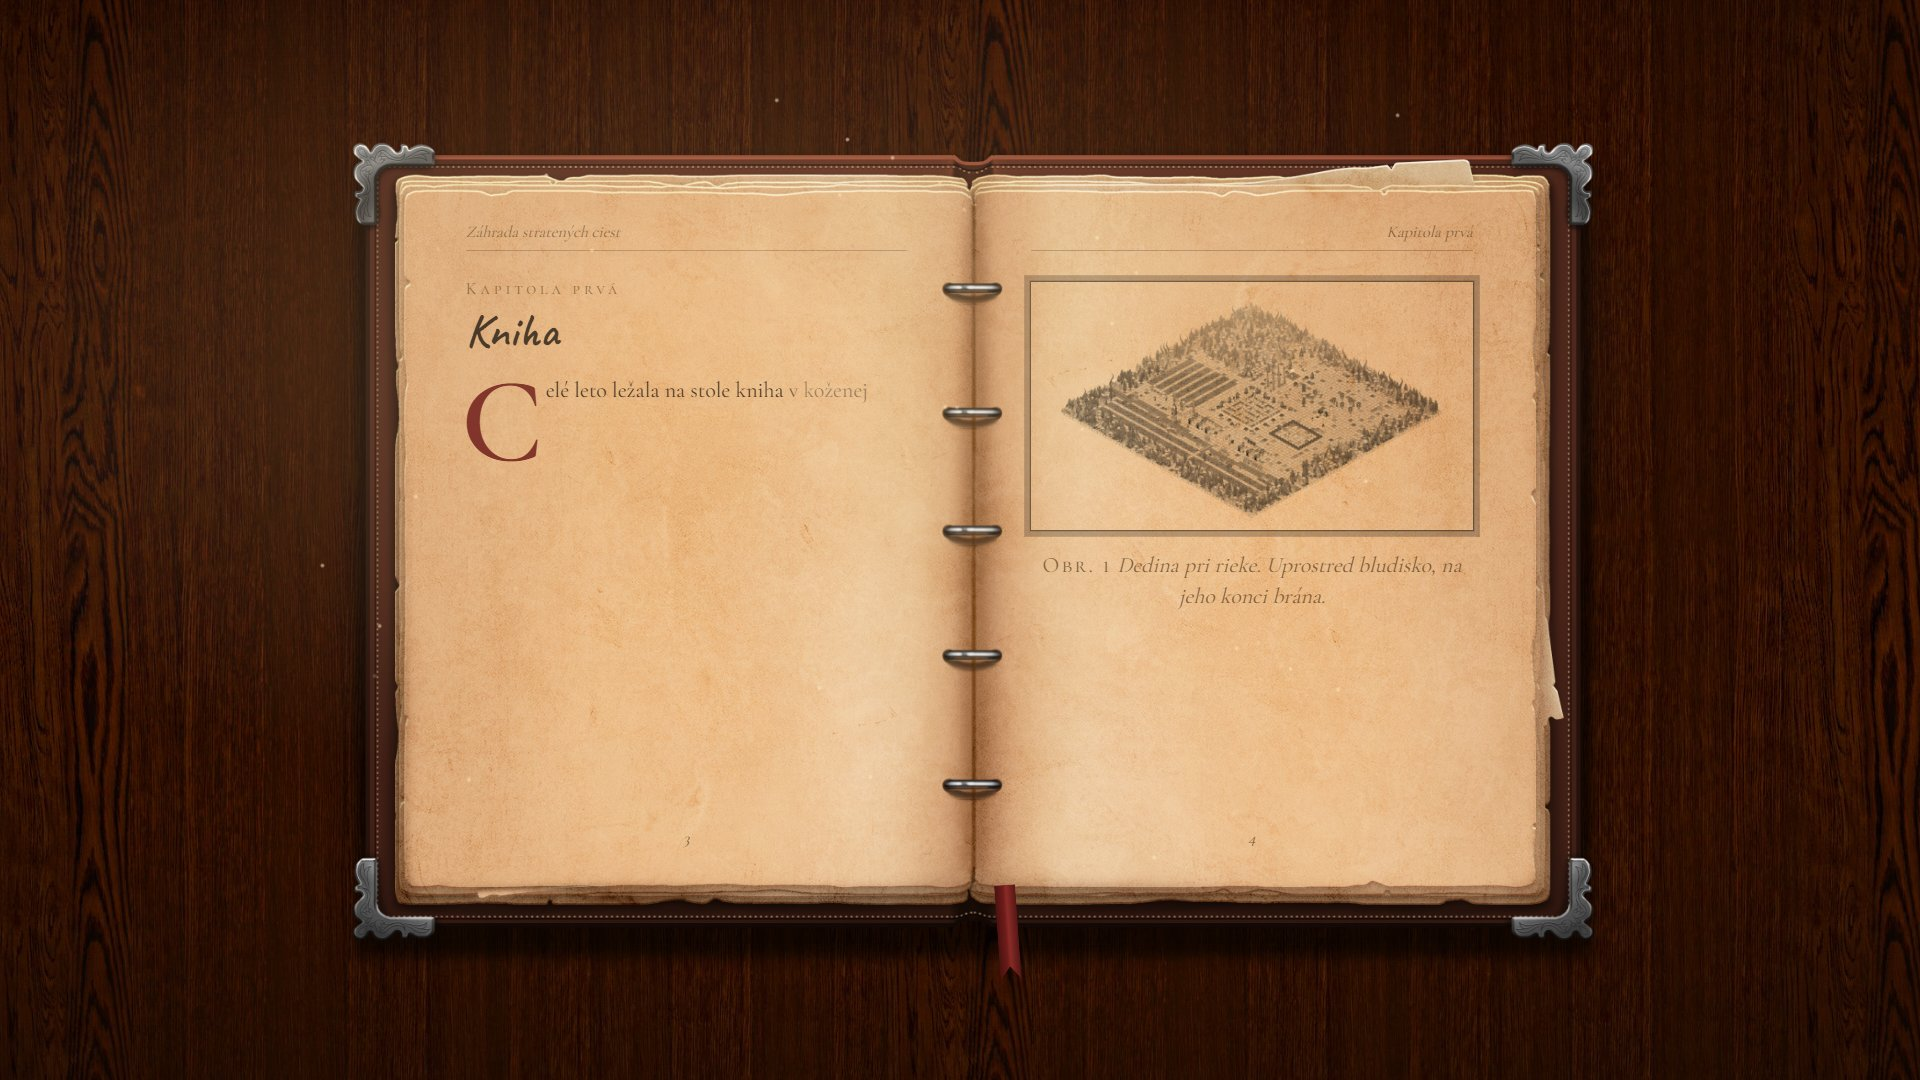
\includegraphics[width=0.85\textwidth]{snimka-prolog-pisanie.jpg}
  \caption{Prológ – kresba sa vpíja do papiera, text sa píše}
\end{figure}

\begin{figure}[H]
  \centering
  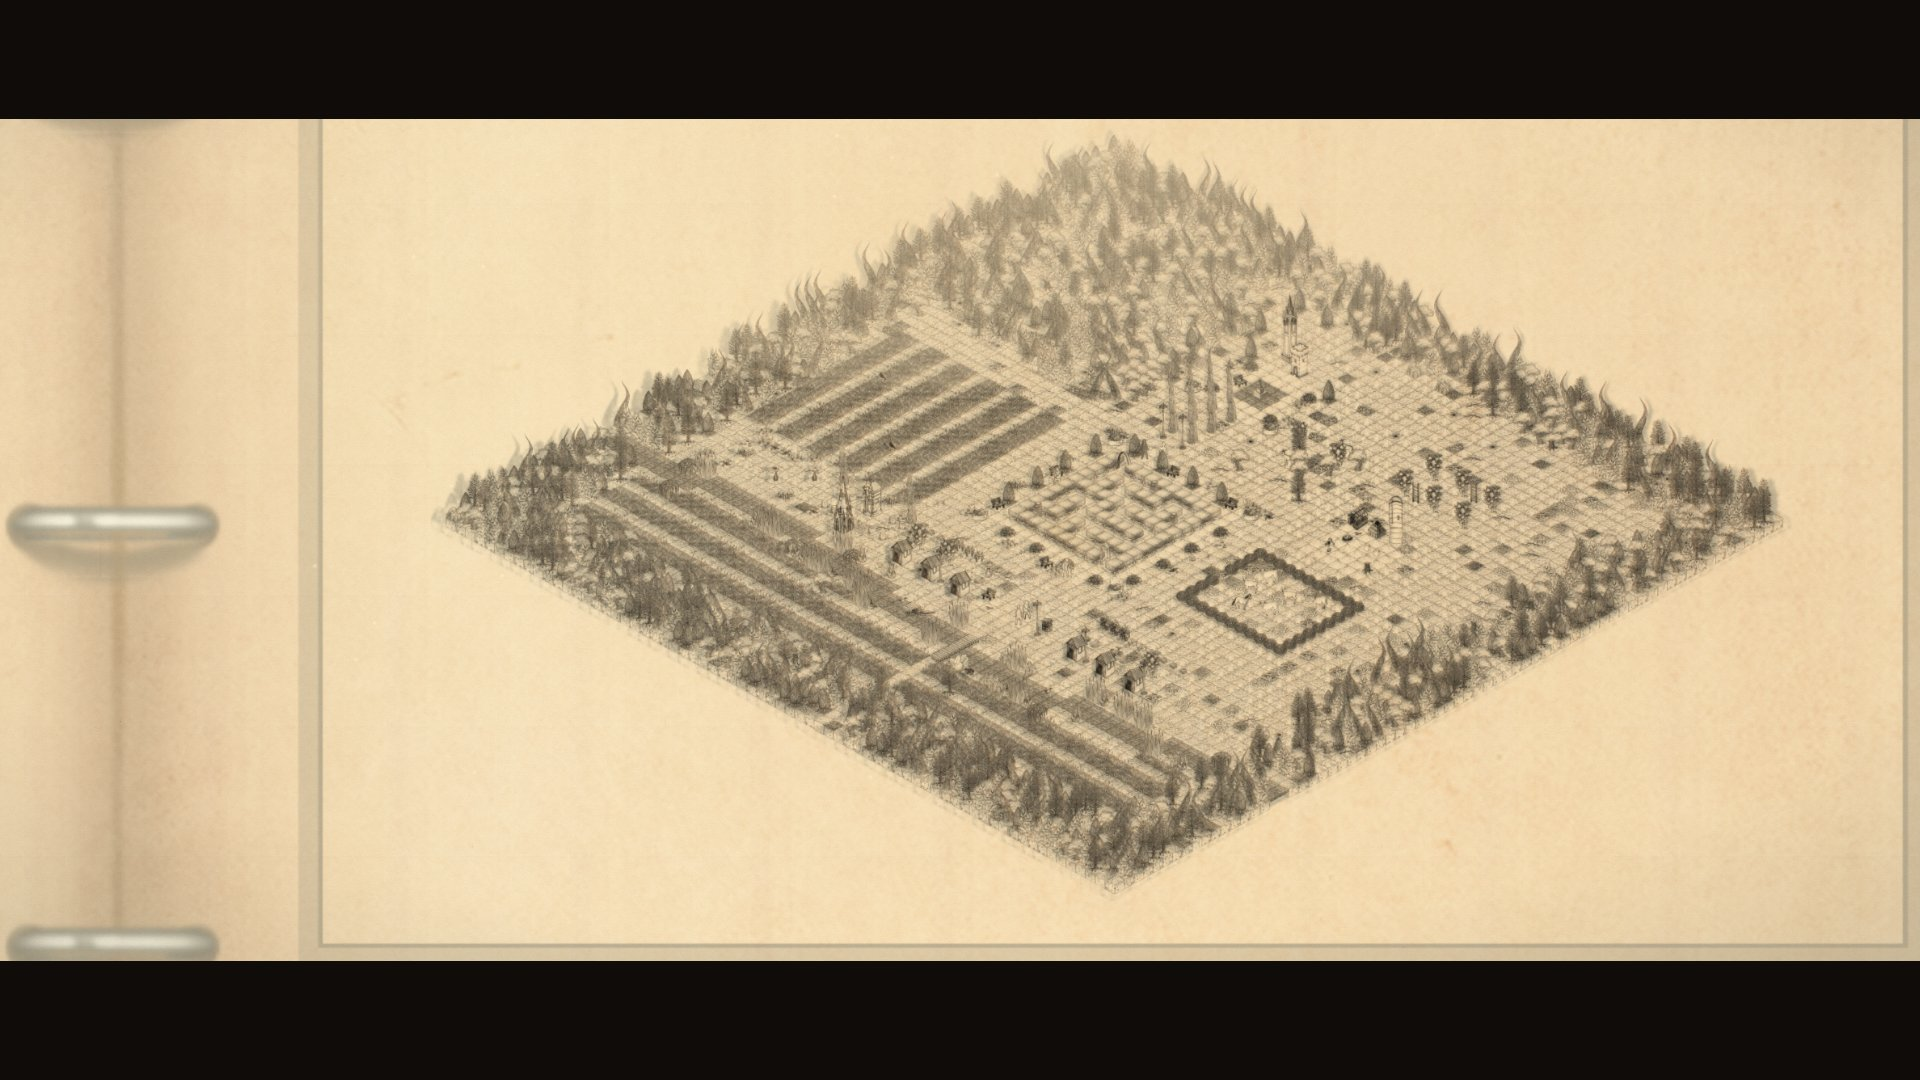
\includegraphics[width=0.85\textwidth]{snimka-let.jpg}
  \caption{Let do kresby: kresba na strane sa mení na živý svet}
\end{figure}

\begin{figure}[H]
  \centering
  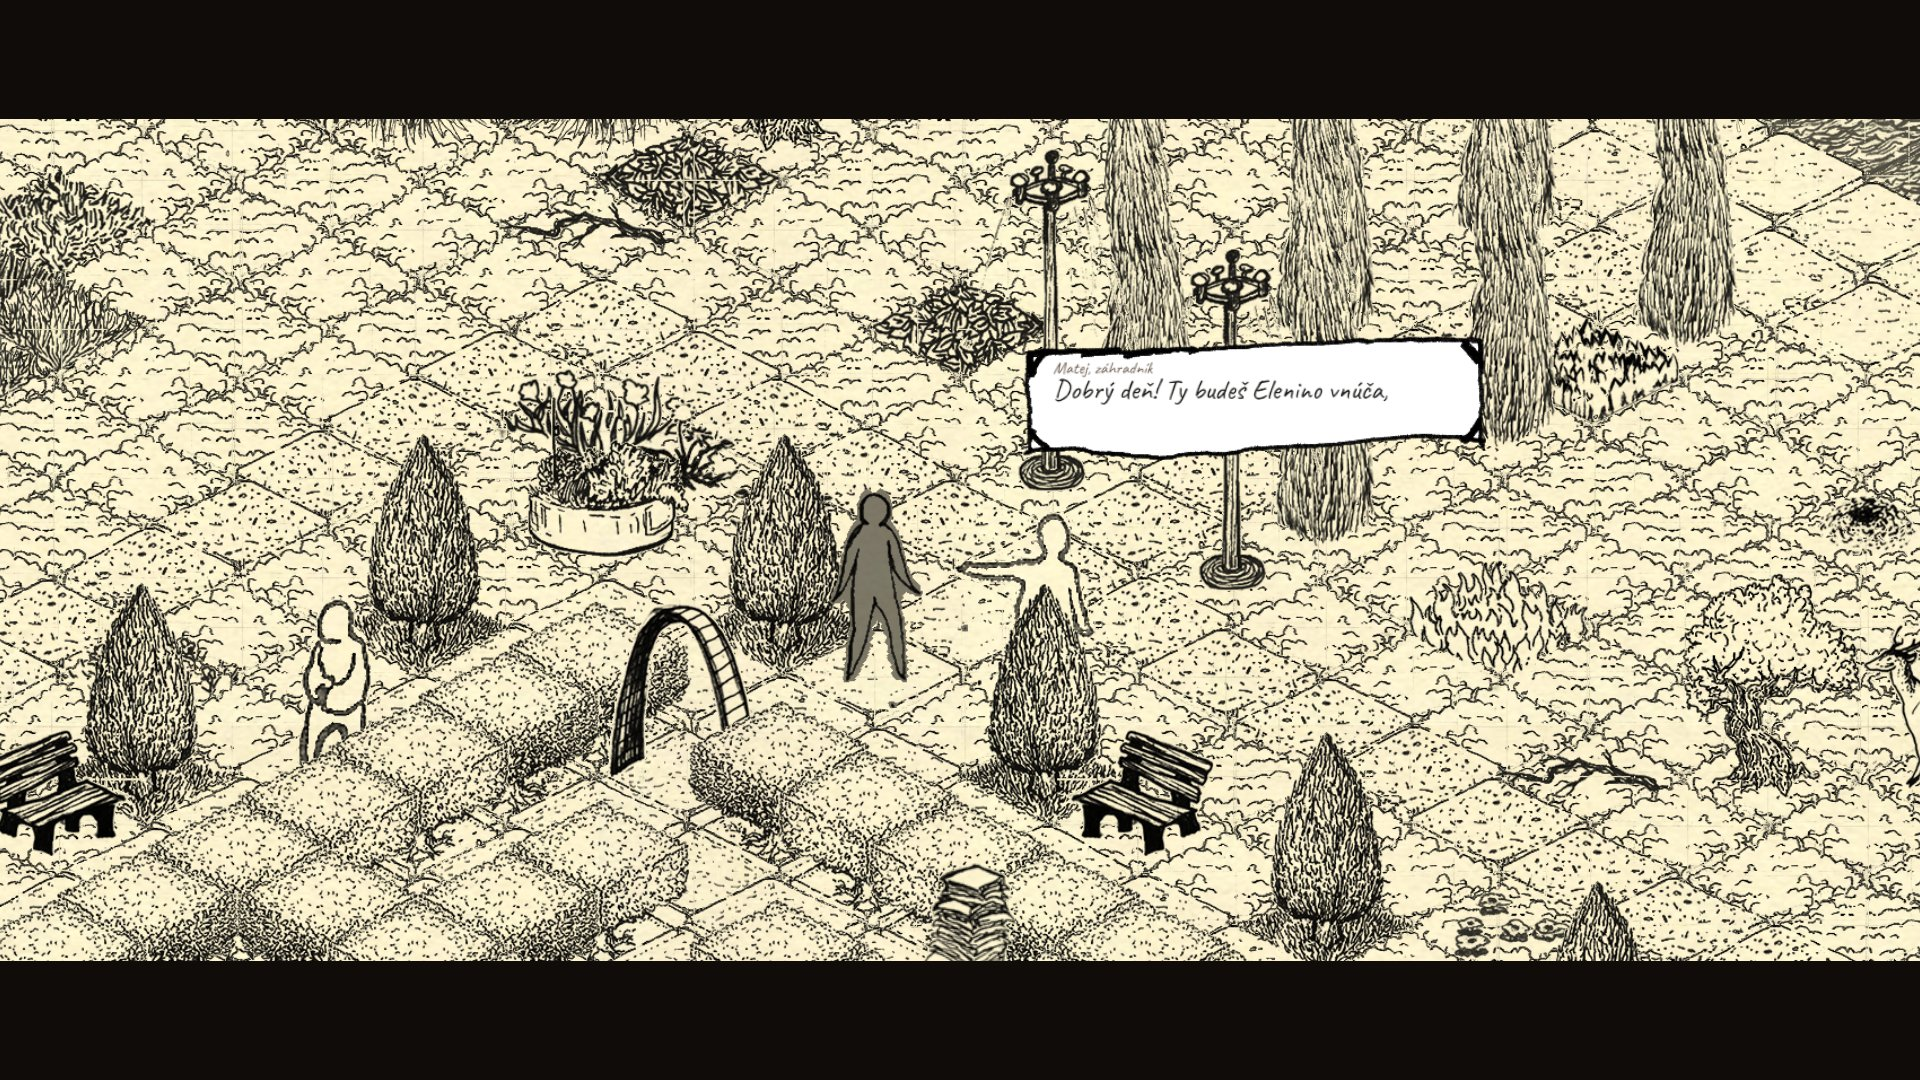
\includegraphics[width=0.85\textwidth]{snimka-zahradnik.jpg}
  \caption{Rozhovor so záhradníkom pri vstupnej bráne}
\end{figure}

\begin{figure}[H]
  \centering
  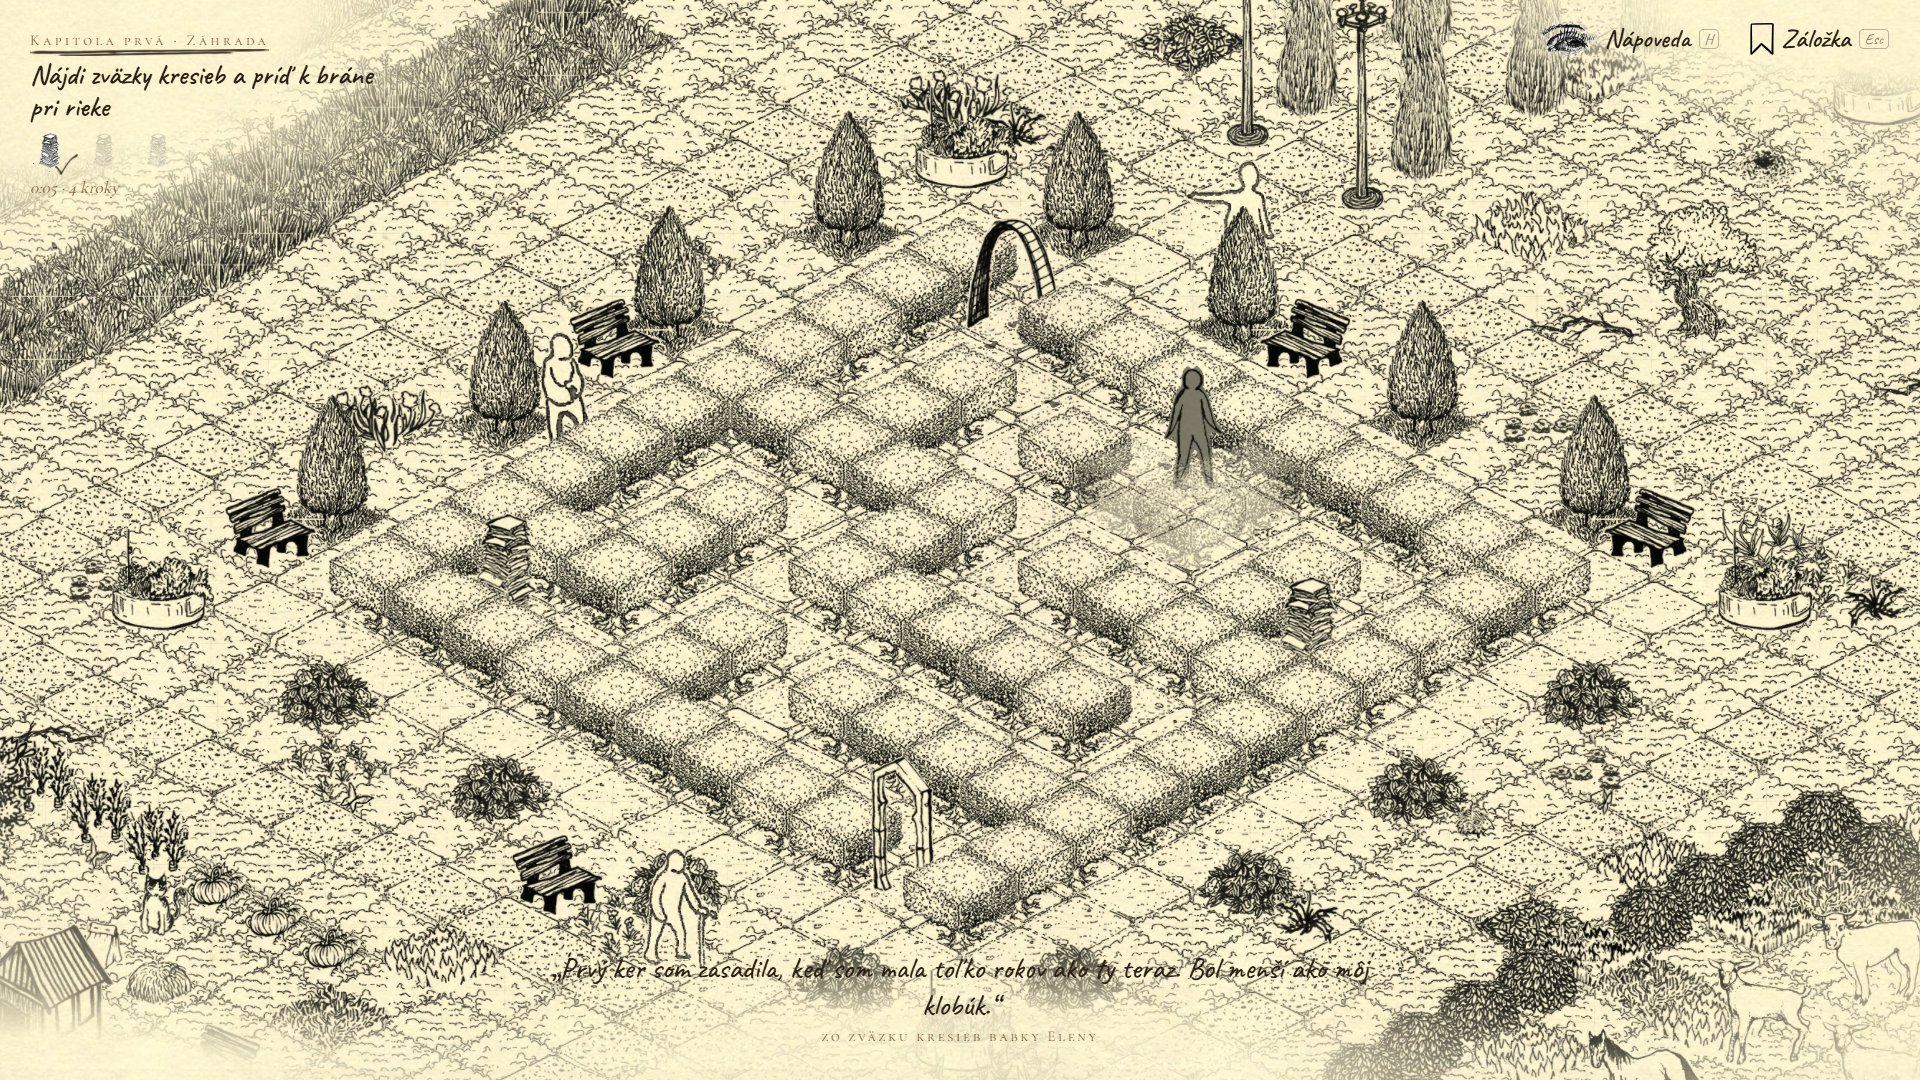
\includegraphics[width=0.85\textwidth]{snimka-zvazok.jpg}
  \caption{Nájdený zväzok kresieb a spomienka v~titulkoch}
\end{figure}

\begin{figure}[H]
  \centering
  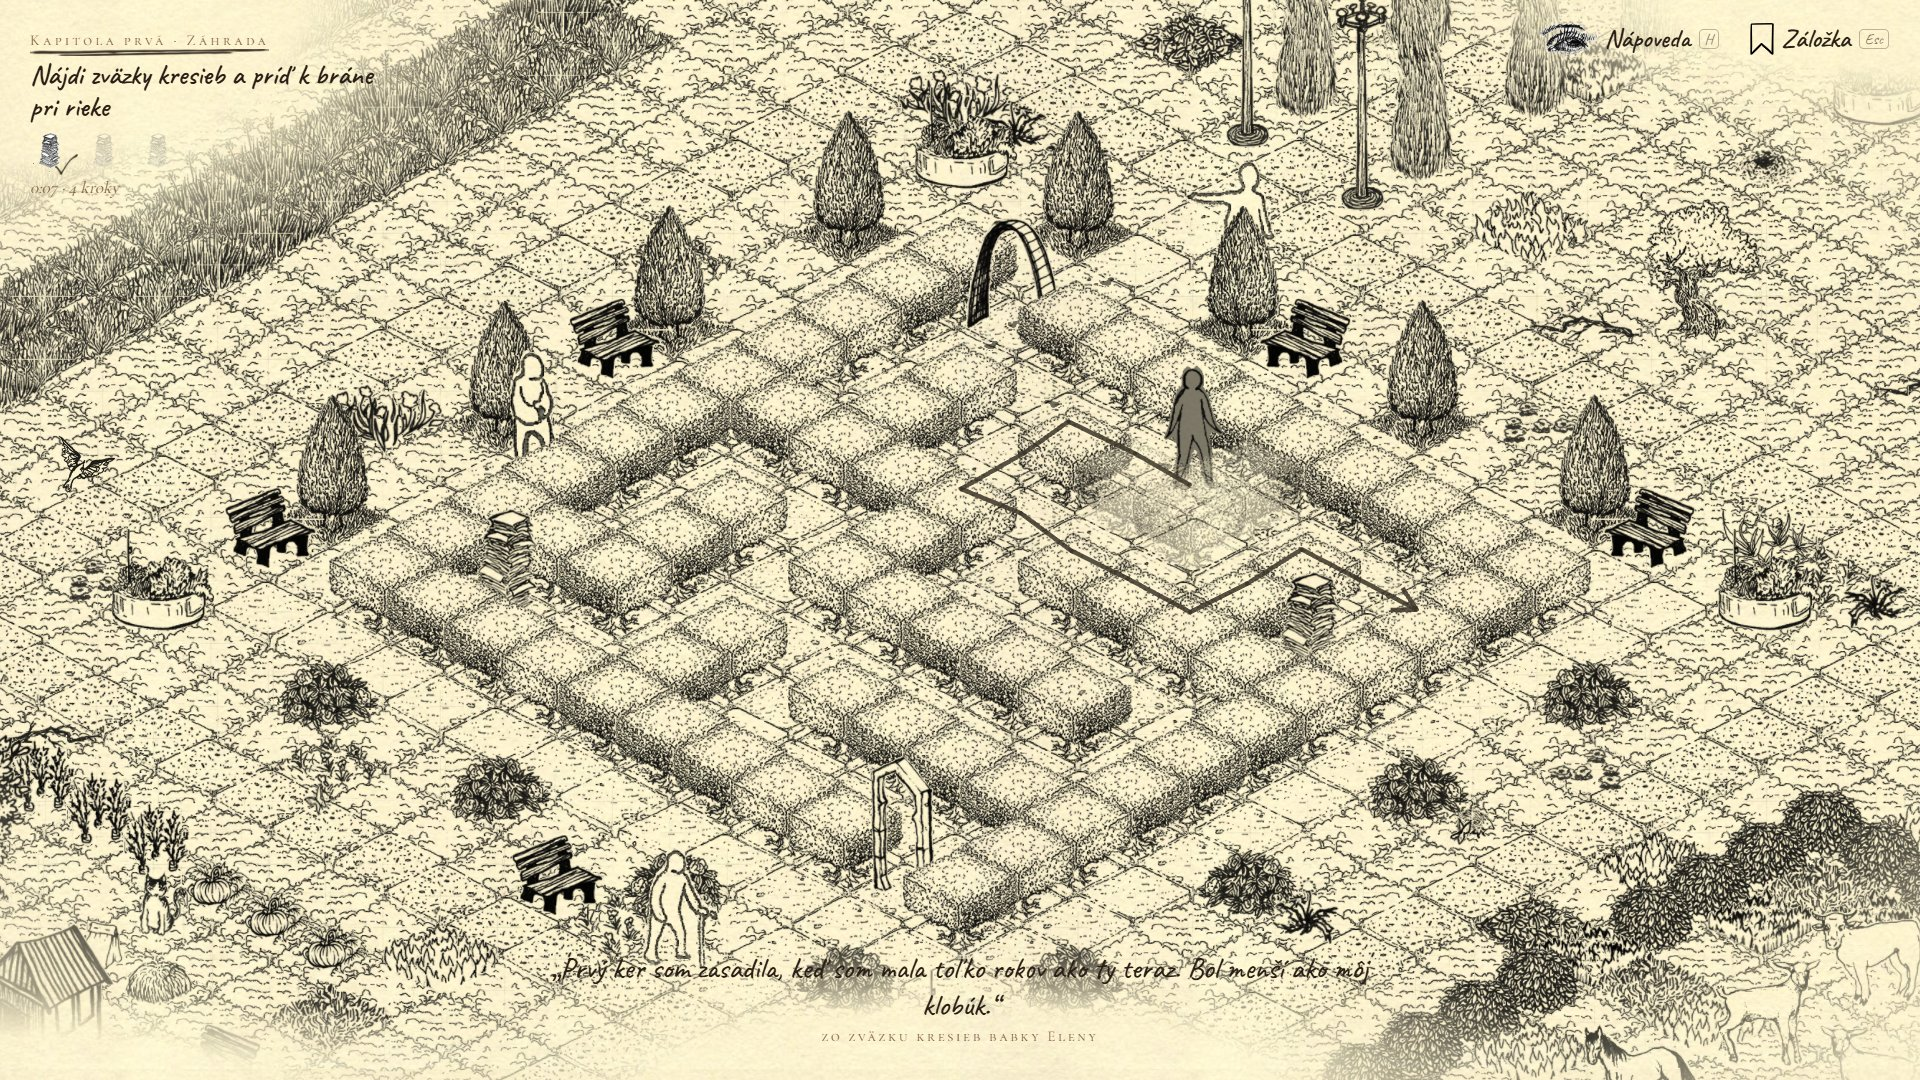
\includegraphics[width=0.85\textwidth]{snimka-napoveda.jpg}
  \caption{Nápoveda: ceruzkou nakreslená cesta k~najbližšiemu cieľu}
\end{figure}

\begin{figure}[H]
  \centering
  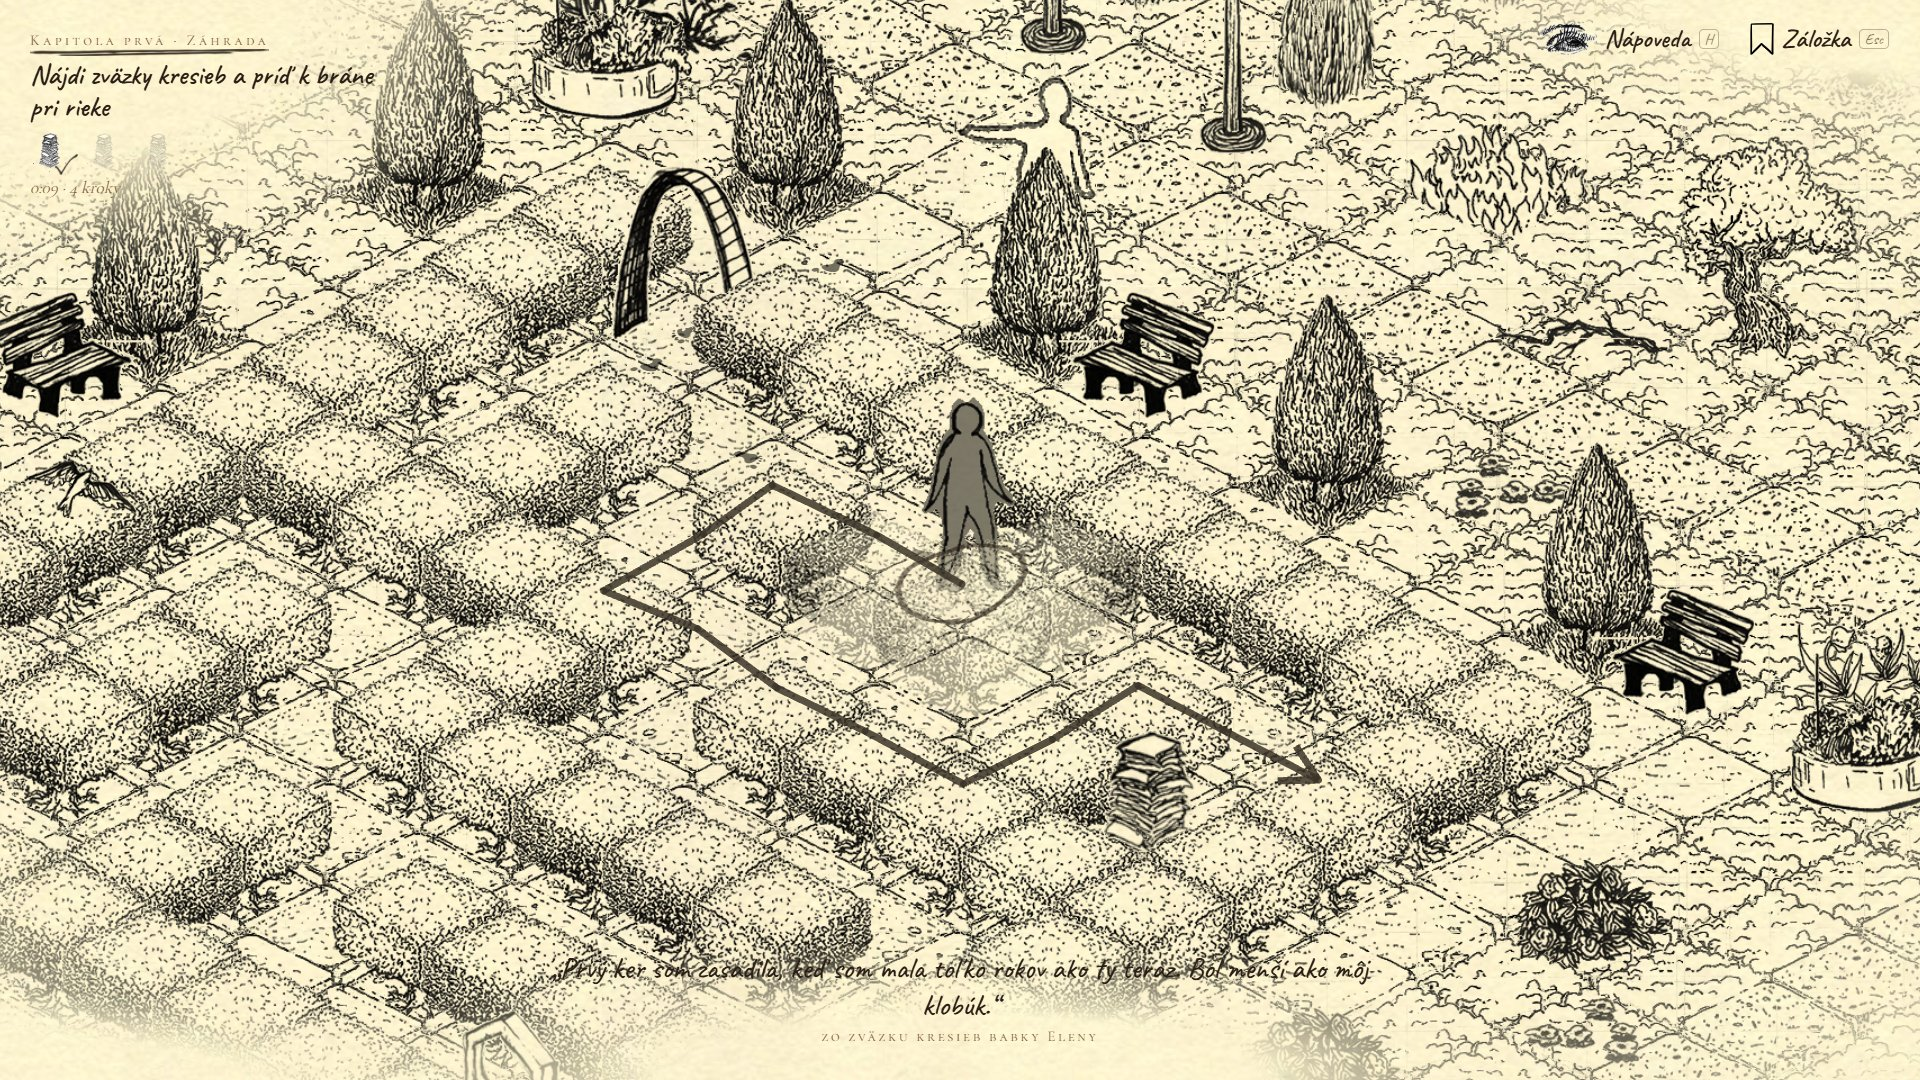
\includegraphics[width=0.85\textwidth]{snimka-priblizenie.jpg}
  \caption{Priblíženie kolieskom myši}
\end{figure}

\begin{figure}[H]
  \centering
  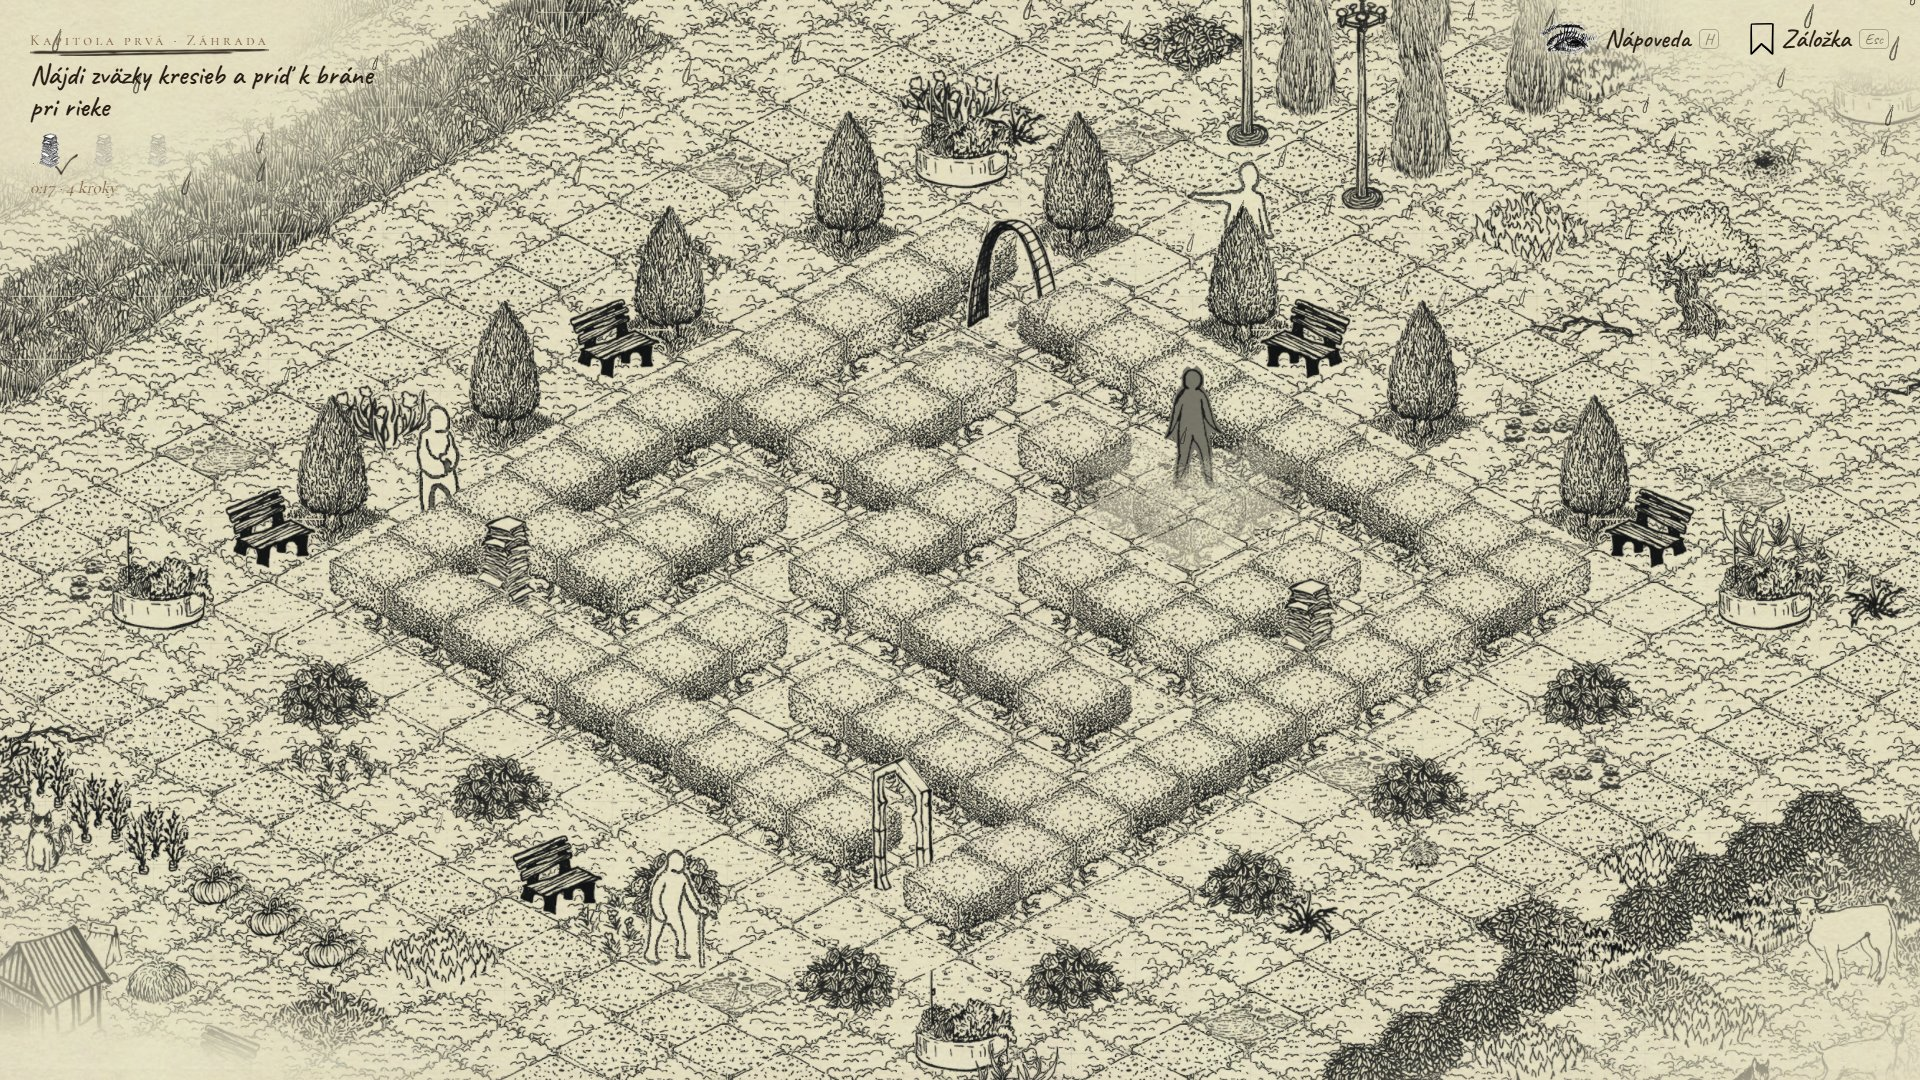
\includegraphics[width=0.85\textwidth]{snimka-dazd.jpg}
  \caption{Dážď v~záhrade}
\end{figure}

\begin{figure}[H]
  \centering
  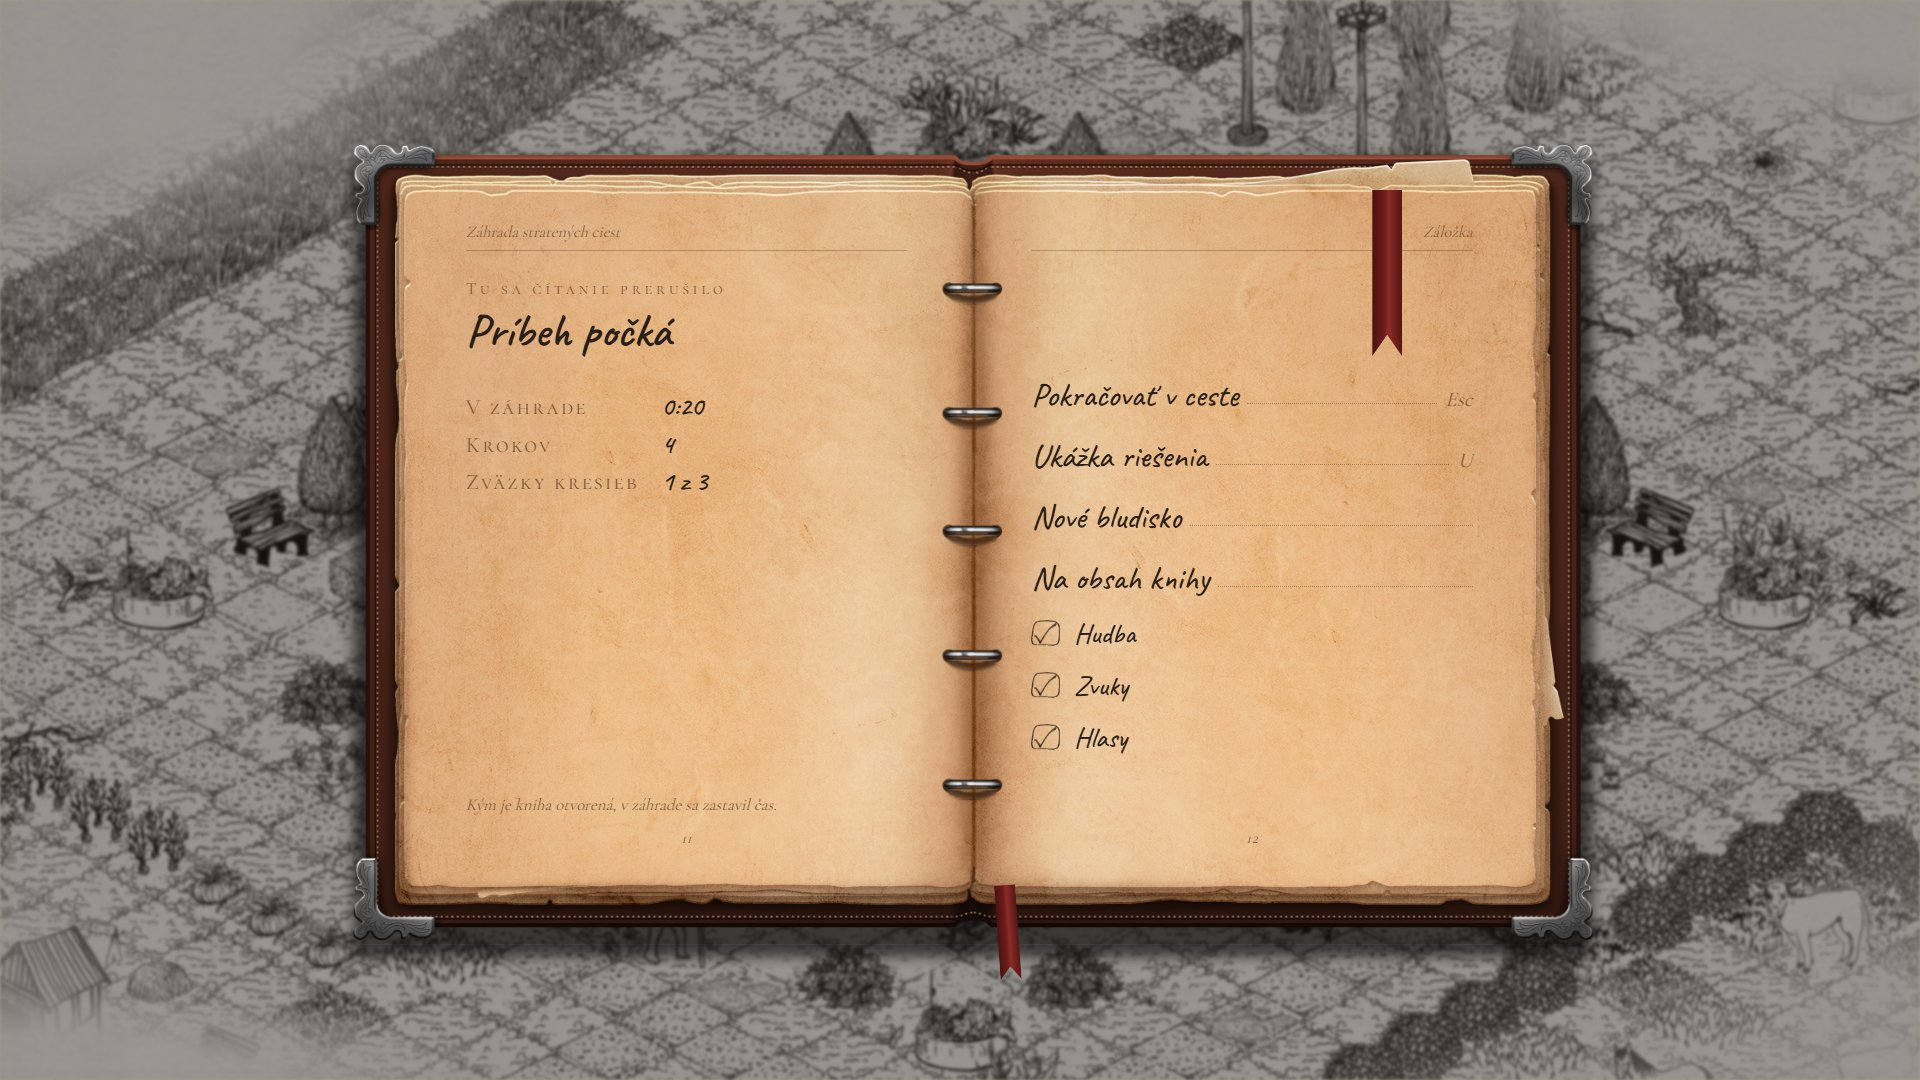
\includegraphics[width=0.85\textwidth]{snimka-zalozka.jpg}
  \caption{Záložka (pauza)}\label{fig:zalozka}
\end{figure}

\begin{figure}[H]
  \centering
  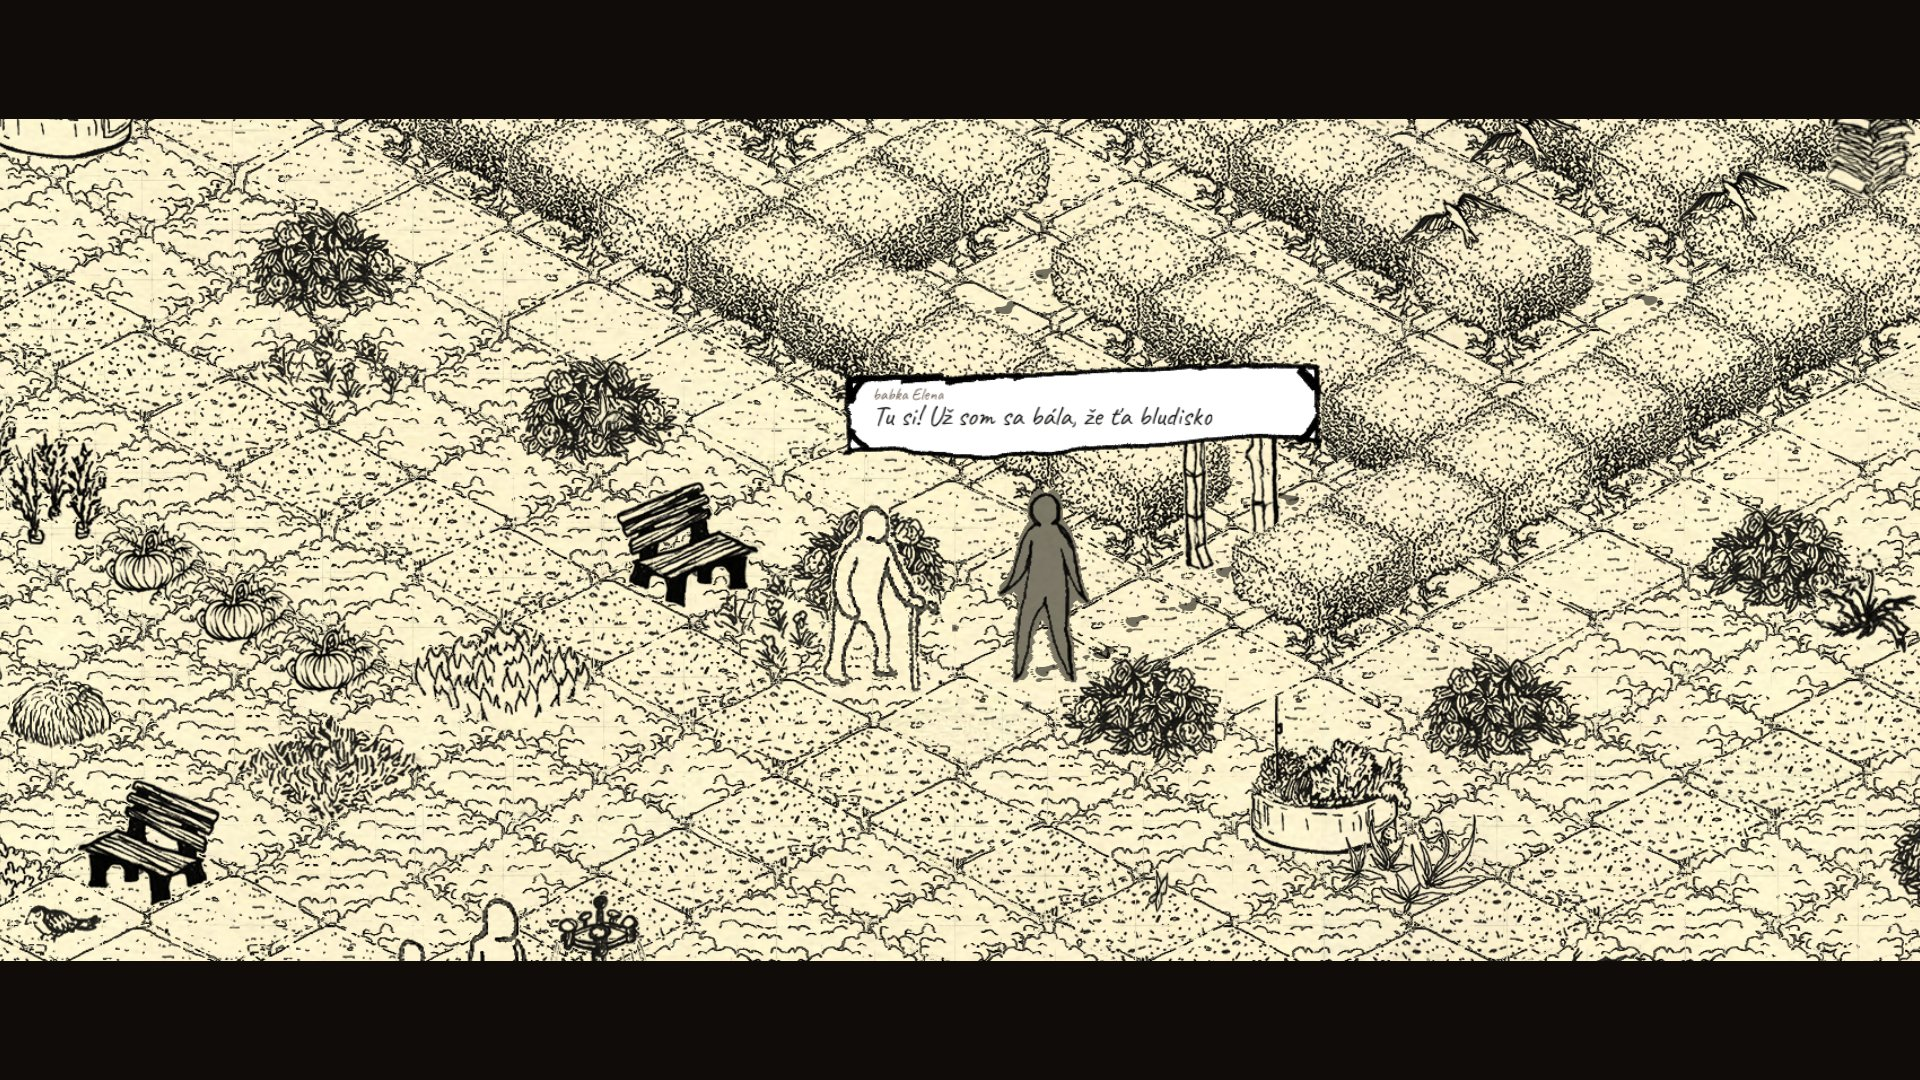
\includegraphics[width=0.85\textwidth]{snimka-babka.jpg}
  \caption{Babka Elena pri výstupnej bráne}
\end{figure}

\begin{figure}[H]
  \centering
  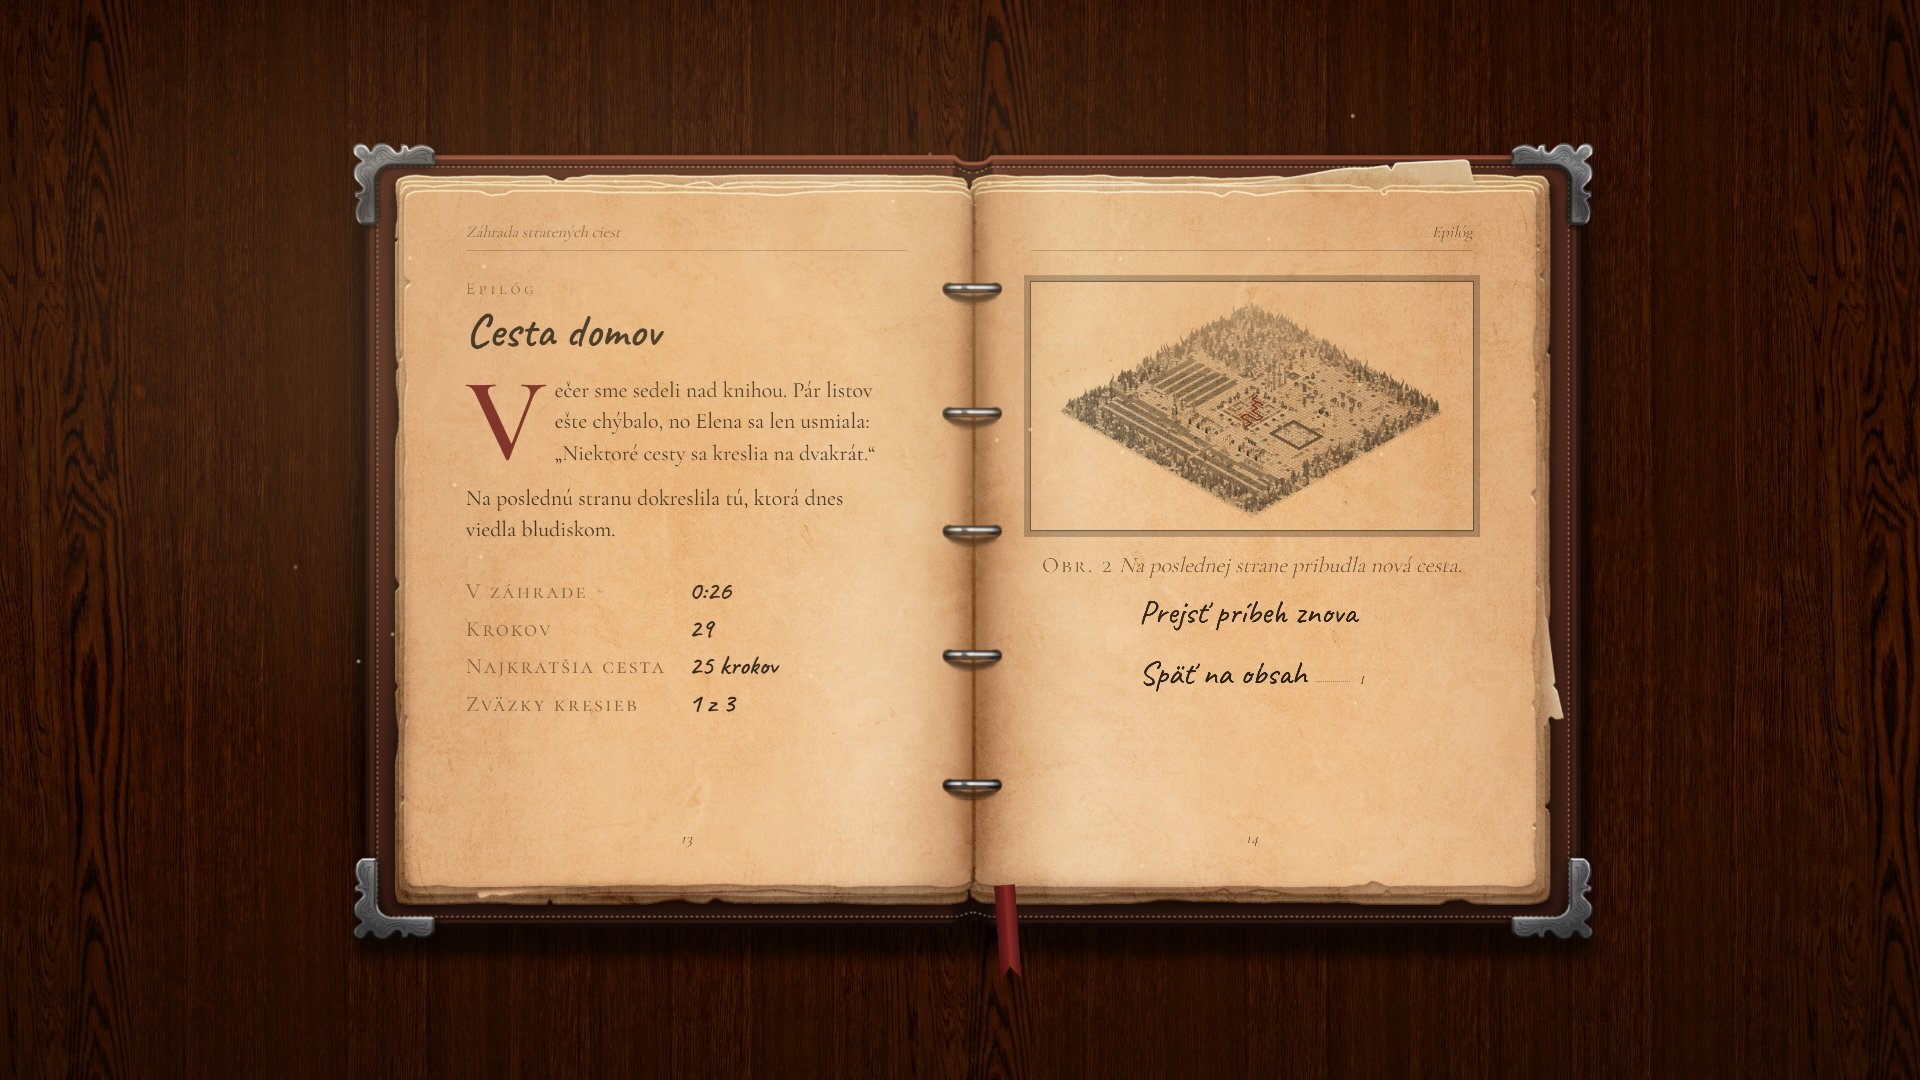
\includegraphics[width=0.85\textwidth]{snimka-epilog.jpg}
  \caption{Epilóg s~výsledkom a nakreslenou cestou}
\end{figure}

\begin{figure}[H]
  \centering
  
\includegraphics[width=0.85\textwidth]{snimka-koniec.jpg}
  \caption{Aplikácia po zavretí knihy}
\end{figure}

\end{document}
